 %%%%%%%%%%%%%%%%%%%%%%%%%%%%%%%%%%%%%%%%%%%%%%
%%%%%%%%%%%%%%%%%%%%%%%%%%%%%%%%%%%%%%%%%%%%%%
%%% Master Thesis Template by Fabian Schär %%%
%%%%%%%%%%%%%%%%%%%%%%%%%%%%%%%%%%%%%%%%%%%%%%
%%%%%%%%%%%%%%%%%%%%%%%%%%%%%%%%%%%%%%%%%%%%%%

%%%%%%%%%%%%%%%%%%%%%%%%%%%%%%%%%%%%%%
%%% Packages and Document Settings %%%
%%%%%%%%%%%%%%%%%%%%%%%%%%%%%%%%%%%%%%

\documentclass[12pt,a4paper,titlepage,oneside,english]{article}

%%% Main Packages %%%
\usepackage[english]{babel}
%\usepackage[ngerman]{babel} % Use this option for German settings.
\usepackage[T1]{fontenc}
\usepackage[utf8]{inputenc}

%%% Additional Packages %%%
\usepackage{cite}
\usepackage{framed}
\usepackage{graphicx}
%\usepackage[german]{fancyref}
\usepackage[german,hidelinks]{hyperref} %hidelinks
\usepackage{multirow}
\usepackage[round]{natbib}
\usepackage{setspace}
\usepackage{geometry}
\usepackage{pst-all} % Not working with Sweave!!!
\usepackage{tikz}
\usetikzlibrary{positioning, intersections}
\usepackage{subcaption}


%%% Math Packages %%%
\usepackage{amsmath}
\usepackage{amstext}
\usepackage{amssymb}
\usepackage{theorem}
\usepackage{epsfig}
\usepackage{longtable}

%%% Layout Specifications %%%
\geometry{a4paper, top=35mm, left=40mm, right=40mm, bottom=45mm,
headsep=10mm, footskip=12mm}

%%% Parskip Settings %%%
\setlength{\parskip}{3mm}
\setlength{\parindent}{0mm}

%%% Document Specifications %%%
\title{Template Master's Thesis}
\author{John Doe}


%%%%%%%%%%%%%%%%%%
%%% Title Page %%%
%%%%%%%%%%%%%%%%%%

\begin{document}
%\begin{titlepage}
\begin{center}
\vspace{1em}
\large{Master Thesis}\\
\huge Developing Address Clustering Heuristics for Account-Based Blockchain Networks:\\ An Analysis based on a Specific Address Set \\
\Large \vspace{1em}
Dario Thürkauf
\end{center}

\vspace{1em}
\normalsize
\begin{flushleft}
Supervised by:\\ 
Prof. Dr. Fabian Schär \\ 
Professor for Distributed Ledger Technologies and Fintech \\
Center for Innovative Finance, University of Basel
\end{flushleft}

\vspace{1em}
\onehalfspacing
\begin{center}
\section*{Abstract}
\end{center}
Assentiar consuetae ha opinionum mentemque ob ii. Ne conflantur de intelligat et me cohibendam. Imaginandi ob to at agnoscerem et mutationum. In methodum ob ii at quicquid lectorum. Procuravi ha dependent ob evidenter tangantur concipere. Immortalem objectivus deo eae rei attingebam ita advertebam quamprimum. Typis patet prius qua nia mem ens. Suppono sim ita pendere nam agnosci quopiam vestiri spondeo dum. Tes illum mundo vetus signa fit talem res his.  \\
\vfill
\textbf{Keywords:} Blockchain, Accounts, Clustering Heuristics, Entity Identification, Graph Representation Learning.\\
%\noindent\textbf{JEL:} X00, X00, X00
%\end{titlepage}


%%%%%%%%%%%%%%%%%%%%%%%%%%%%%
%%% Contents & Declaration%%%
%%%%%%%%%%%%%%%%%%%%%%%%%%%%%

\pagenumbering{gobble}

\newpage
\pagenumbering{Roman}
\tableofcontents

\vfill
\begin{center}

\includegraphics[width=4cm]{../figures/logo_cif.png}
\end{center}
\newpage
\singlespacing
%\vspace{-1.5cm}
\section*{Declaration of Independent Authorship}
I attest with my signature that I have written this work independently and without outside help. I also attest that the information concerning the sources used in this work is true and complete in every respect. All sources that have been quoted or paraphrased have been marked accordingly. 
Additionally, I affirm that any text passages written with the help of AI-supported technology are marked as such, including a reference to the AI-supported program used. This paper may be checked for plagiarism and use of AI-supported technology using the appropriate software. I understand that unethical conduct may lead to a grade of 1 or ``fail`` or expulsion from the study program.\\

Dario Thürkauf

\begin{figure}[h!]
	\centering
	\hspace{-10cm}
	
\includegraphics[width=3cm]{../figures/signature.jpeg}
\end{figure}
%%%%%%%%%%%%%%%%%%%%

\newpage
\onehalfspacing
\pagenumbering{arabic}


%%%%%%%%%%%%%%%%%%%
%%% Introduction%%%
%%%%%%%%%%%%%%%%%%%

\section{Introduction}

Public permissionless blockchains such as Bitcoin \citep{nakamotoBitcoin2008} and Ethereum \citep{buterin2014ethereum} allow users %individuals
 to participate with multiple pseudonymous addresses, the creation of which is virtually cost-free. Contrary to popular belief, these blockchains are entirely transparent. All transactions are publicly observable and stored as part of the blockchain's history.
This circumstance has opened up a nascent scientific field dealing with entity identification within blockchain networks. Researchers try to cluster addresses controlled by the same user by analyzing on-chain data and detecting usage patterns. The frequent lack of ground truth makes it difficult to evaluate different clustering methods. As a result, most methods are heuristic. %The majority of these methods are heuristic which often makes them difficult to evaluate due to the absence of any ground truth.
\newline On one hand, identifying addresses that belong to the same real-world entity is beneficial as it allows for better evaluation of network properties concerning usage, distribution of wealth, and detecting fraudulent activities \citep{FV:17}. For instance, if a user distributes their voting power across various addresses, they might manipulate an on-chain voting process that seems fair at the outset. \newline
Conversely, the lack of privacy is also detrimental to most financial use cases. As a response, multiple privacy-enhancing tools and protocols have been proposed to obfuscate transaction tracing. 
Nonetheless, these protocols have yet to be widely adopted, and careless user behavior can undermine the privacy guarantees they offer. \newline
With these considerations in mind, the topic of privacy, or lack thereof, will remain significant for future blockchain development and research.
%If someone obtains information that allows them to link a blockchain address to an entity, they may effectively observe that entity’s entire transaction history and associated activity. Even if the entity uses multiple addresses, any link between these addresses may expose the fact that they belong to the same person.

\textbf{Related work}\\
Previous work in this field can be broadly distinguished between methods developed for the unspent transaction output (UTXO) model (e.g., Bitcoin and ZCash) and the account-based model (e.g., Ethereum and Polygon). While both models share the concept of addresses, the notion of accounts is absent in UTXO-based blockchains. The way in which transactions are processed is fundamentally different, and therefore, clustering heuristics are not applicable to both paradigms.

Several address clustering heuristics in the UTXO setup have been proposed for Bitcoin and its derivatives \citep{Androulaki2013, Meiklejohn2013, Haslhofer2016, jourdan2018, kappos2022}. However, these methods are outside the scope of this work and will not discussed. \newline 
As suggested by \cite{nakamotoBitcoin2008} in the Bitcoin whitepaper, most Bitcoin wallet implementations use a new key pair for each transaction to keep them from being linked to a common owner. Unlike the UTXO model, native transactions in account-based blockchains can only move funds between a single sender and receiver, and the ``change`` remains in the sender account. Subsequent transactions necessarily use the same address again. The account-based model essentially relies on address reuse at the protocol level \citep{Beres2020}. Consequently, privacy guarantees should be lower as participants typically use a limited set of addresses. \newline
% Make an assumption that people only use a small set of addresses
Clustering heuristics for account-based blockchains were first introduced by \cite{FV:17}. He proposed and applied heuristics that exploit patterns related to deposit addresses, multiple participation in airdrops, and token authorization mechanisms. \newline
\cite{Beres2020} propose more universally applicable methods, arguing that Victor’s heuristics, while powerful, assume participation in certain on-chain events. Their approach interprets transactions or token transfers as network graphs, with addresses as nodes and asset transfers as edges. They quantitatively compare graph-representation learning algorithms (a subset of machine learning) and propose further user profiling techniques based on time-of-day activity and transaction fee patterns. Using ENS address pairs as ground truth, the authors rigorously test their methods and apply their findings to significantly reduce the privacy guarantees of \textit{Tornado Cash}, a non-custodial privacy-enhancing protocol on Ethereum. \newline
\cite{wu2022tutela} extend on one of \cite{Beres2020} graph representation learning algorithms and apply it at scale. Further, they also propose a set of new clustering heuristics targeting Tornado Cash,  showing that careless user behavior can still reveal identity. Based on those heuristics, they developed an application to measure the anonymity of an Ethereum address. All of the aforementioned methods will be discussed in greater depth in Section 3. \newline
Broadening the scope of entity identification, \cite{victorlüders2019} study the largest Ethereum ERC-20 token networks from a graph perspective. Similarly, \cite{casalebrunet2021} apply network graph analysis to various non-fungible token (NFT) ecosystems. Both find that many networks follow a star or a hub-and-spoke pattern, similar to social network interaction graphs. Moreover, \cite{Payette2017} propose a segmentation of the Ethereum address space into four distinct behavior groups sharing similar attributes while applying k-means clustering. \newline
Rather than treating users as entities and analyzing on-chain data, \cite{yu2023} propose a novel approach for correlation analysis by exploiting network information. Although this approach can potentially avoid the impact of privacy-enhancing technologies, it introduces new limitations and problems. Thus, this method may be of great interest for future research, particularly when privacy-enhancing techniques become more widely used.

\textbf{Our contribution}\\
In this work, we perform entity identification on an address set containing 473,927 addresses. To obtain these addresses, a separate project collected snapshots of avatar activity in Decentraland over nine months from July 2022 to April 2023. Due to Decentraland's blockchain-based architecture, each avatar contains information about a user's Web3 address. \newline
We test the applicability of existing heuristics, and if feasible, their efficacy in detecting entities using multiple addresses is evaluated.
The main objective is to estimate the number of real-world entities these addresses represent. The clustering of addresses is limited to this set only, without considering any addresses outside of it, e.g., that were not registered in Decentraland during the given time frame. Furthermore, we introduce our heuristic for identifying address clusters and evaluate its suitability for implementation in other contexts. As of our knowledge, we are the first to cluster addresses within a predefined set on a large scale.
%Anwenden/discuss/anpassen/erweitern and evaluate existing heuristics to my specific address set.

The remainder of this paper is structured as follows: In Section 2, we provide a brief overview of the basic concepts necessary to understand the setup, including Ethereum accounts, tokens, Decentraland, and privacy-enhancing protocols. Section 3 describes our methodology for data collection and preparation. The fourth section provides a detailed explanation of various clustering heuristics. The fifth section applies the clustering heuristics described in section 4, after which we discuss the results of our analysis and summarize our findings in sections 6 and 7.

%%%%%%%%%%%%%%%%%%%%%
%%% Preliminaries %%%
%%%%%%%%%%%%%%%%%%%%%

\section{Preliminaries}

\subsection{Contract Accounts and EOAs}
Account-based blockchains usually distinguish between externally owned accounts (EOAs) and contract accounts (smart contracts). \textit{EOAs} are created and controlled by private keys and can be used to hold the native protocol asset, send and receive transactions, and interact with contract accounts. \textit{Contract accounts} are controlled by the contract's code, their state can be modified through transactions sent to the contract and they cannot initiate transactions. \citep{buterin2014ethereum} \newline Each account has a 20-byte address encoded in hexadecimal. For EOAs, this address is based on the last 20 bytes of the Keccak-256 hash of the ECDSA public key. For contract accounts, it is usually the last 20 bytes of the Keccak-256 hash of the RLP encoding of the sender address and account nonce. \citep{GW:14}

\subsection{Ethereum, Polygon and the EVM}
Ethereum and Polygon are both smart contract-based account-model blockchains. They share the same execution logic - the Ethereum Virtual Machine (EVM).
The EVM provides a standardized framework for contract execution, ensuring that smart contracts produce deterministic results across all nodes in the network \citep{GW:14}. The EVM is independent of the underlying blockchain protocol, allowing other blockchain implementations to adopt this standardized framework for contract execution.\newline
\textit{Polygon} is a so-called sidechain and aims to address the scalability limitations of Ethereum. The adoption of the EVM means that both blockchains share the same user address schemes. It also enables developers to deploy and execute Ethereum-based smart contracts on the Polygon network with minimal changes. \citep{matic_whitepaper}
%A high-level programming language is typically used to write smart contracts, and a compiler to convert them into bytecode \citep{mastering_ethereum}

\subsection{Tokens and Token Standards}
\cite{roth2019tokenization} define \textit{tokens} as rivalrous, digital units of value that represent ownership of an asset or utility. Smart contracts are the primary method of creating tokens on EVM-based blockchains. In essence, a smart-contract-based token is a mapping of accounts with token balances and a set of functions defining how these balances can be changed. Any smart contract containing these elements can be interpreted as a token contract. \citep{roth2019tokenization} \newline
\textit{Token standards} specify basic interfaces that allow for interoperability between smart contracts. These standards do not prescribe an implementation but set minimum requirements without restricting the design beyond that \citep{mastering_ethereum}. 
The most common token standards are ERC-20\footnote{\url{https://eips.ethereum.org/EIPS/eip-20}} for fungible tokens, ERC-721\footnote{\url{https://eips.ethereum.org/EIPS/eip-721}} for non-fungible tokens (NFTs) and ERC-1155\footnote{\url{https://eips.ethereum.org/EIPS/eip-1155}} for semi-fungible tokens.\newline
When a transaction completes, it produces a transaction receipt  that contains log entries providing information about the actions that occurred during its execution. Solidity\footnote{Solidity is the dominant high-level programming language for smart contracts targeting the EVM.} high-level objects called ``Events`` construct these logs, which can be queried from a full node and are stored separately from the state. \citep{mastering_ethereum} \newline
The standarization of tokens allows us to listen for ``transfer events``, which are emitted whenever an token changes ownership.
These transfer events include the \textit{sender} and \textit{recipient} address, along with a \textit{token ID} and/or \textit{amount}. 

\subsection{Decentraland}
\textit{Decentraland} is the first large-scale blockchain-based virtual world, with well-known companies like Tommy Hilfiger, Samsung, PepsiCo, Diesel, Adidas, and Netflix actively engaging in it \citep{metaverse-retailing2023}.\newline
Two main reasons make Decentraland an ideal platform for empirical research.
\textit{First}, its open architecture allows compiling snapshots of user activity, including the users' location within the metaverse and Web3 address. Using this capability, \cite{metaverse-retailing2023} captured snapshots of avatar locations over a nine-month period and provided the Web3 addresses collected for this thesis.\newline
\textit{Second}, users who connect their Web3 account can own various digital assets, such as monetary units, land parcels, and avatar collectibles (e.g., wearables, emotes, and names). Smart contracts on Ethereum and Polygon track and manage the ownership of these assets \citep{goldbergschaer2023}. This allows us to analyze the entire transaction history and derive information about the avatars' economic activity. \newline
Initially, Decentraland launched with two native tokens. \textit{LAND}, an NFT compliant with ERC-721, manages the ownership of land parcels in Decentraland. \textit{MANA}, a fungible token compliant with ERC-20, is the in-world currency used to purchase digital goods and services. The majority of purchases and trades are settled in MANA. \newline 
Moreover, the Decentraland core developers provide a smart-contract-based marketplace where users can buy or trade LAND or other in-game collectibles.
%The term metaverse refers to Neal Stephenson’s 1992 novel Snow Crash and describes an immersive virtual world that is populated by humans-as-avatars.

\subsection{Non-custodial crypto asset mixers}
According to \cite{nadler2023tornado}, crypto-asset mixers are currently the most widely used approach to achieve privacy on public blockchains. At a high level, we can distinguish between custodial and non-custodial crypto-asset mixers. \newline
In the custodial setup, users send their assets to a centralized service provider's public deposit address. After some delay, the provider returns the assets to a privately relayed recipient address. This approach is fully trust-based, as the service provider has complete control over the assets and access to the identifying data. \citep{nadler2023tornado} \newline 
In contrast, non-custodial crypto asset mixers (e.g., Tornado Cash) replace the trusted mixing party with a publicly verifiable smart contract. They rely on cryptographic schemes that allow anyone to prove and independently verify the validity of a withdrawal without disclosing the link to a specific deposit. This approach has the advantage that users do not have to share the identifying information with anyone, and there is no liquidity risk as the funds are locked. \citep{nadler2023tornado} \newline
In a nutshell, the mixer works in the following way: Various entities deposit the same amount of a specific crypto asset to a mixer address acting as a pool. Anyone who has contributed to the pool may then generate a new address and withdraw their funds without revealing the link between the deposit and withdrawal addresses. This is achieved using zkSNARKs (zero-knowledge, succinct, non-interactive argument of knowledge). 
Each depositor inserts a hash value in a Merkle tree. At the time of withdrawal, each legitimate withdrawer can prove unlinkably with a zero-knowledge proof that they know the pre-image of a previously inserted hash leaf in the Merkle tree. %Subsequently, users can withdraw their assets from the mixer whenever they consider that the size of the anonymity set is satisfactory.
 For a more detailed description of how Tornado Cash works, see \cite{nadler2023tornado} or \cite{Beres2020}. \newline
In the context of this thesis, it is sufficient to know that third parties can still observe the addresses that have deposited to and withdrawn from the pool. The set of all deposits that a particular withdrawal could be originated from is defined as the \textit{anonymity set}. 
In theory, a larger anonymity set will provide a higher level of privacy since any withdrawal address could be linked to more deposit addresses. However, in practice, this does not always hold.
Some users reveal the link between their withdrawal and deposit addresses, which also affects the privacy of other depositors, for example, by withdrawing from the pool with the same address they deposited or directly sending funds between the two addresses. According to \cite{nadler2023tornado}, careless use of the protocol, testing transactions, or external incentive mechanisms might be reasons for this behavior. \newline
In addition, \cite{Beres2020} and \cite{wu2022tutela} propose approaches to de-anonymize Tornado cash transactions using various clustering heuristics. These methods are discussed in more detail in section 4.
%In theory, a larger anonymity set will provide a higher level of privacy as third parties will not be able to link a specific depositor address to a specific withdrawal address. However, this is not always the case. For example, some users (might) withdraw from the pool with the same address as they deposited. According to \cite{nadler2023tornado}, careless use of the protocol, testing transactions or external incentive mechanisms might be reasons for this behaviour. \newline
%In addition, \cite{Beres2020} and \cite{wu2022tutela} propose approaches to de-anonymize Tornado cash transactions using various clustering heuristics. These methods are discussed in more detail in section 4.
%it is more difficult to link a withdrawal address to a specific depositor address)
%making use of address re-use, transaction activity, transaction cost choice, or more complex transaction graph and network analyses.


%%%%%%%%%%%%
%%% Data %%%
%%%%%%%%%%%%

\section{Data Collection and Preparation} 
The starting point for our work was a data set comprising 473,927 distinct Web3 addresses. %The original data set comprised 473,927 distinct (Web3) addresses.
 As we focus on clustering methods using on-chain data, we exclude addresses that have not been recorded on either Ethereum or Polygon. To accomplish this, we used data from Blockscan\footnote{\url{https://blockscan.com/}}. Overall, 59,651 addresses were recorded on Ethereum, 129,988 on Polygon, with 52,095 addresses appearing on both networks simultaneously. The set of ``clusterable`` addresses therefore counts 137,544 addresses. The subsets are visualized as a Venn diagram in Figure \ref{fig:Venn}.
 
\begin{figure}[h!]
	\centering
	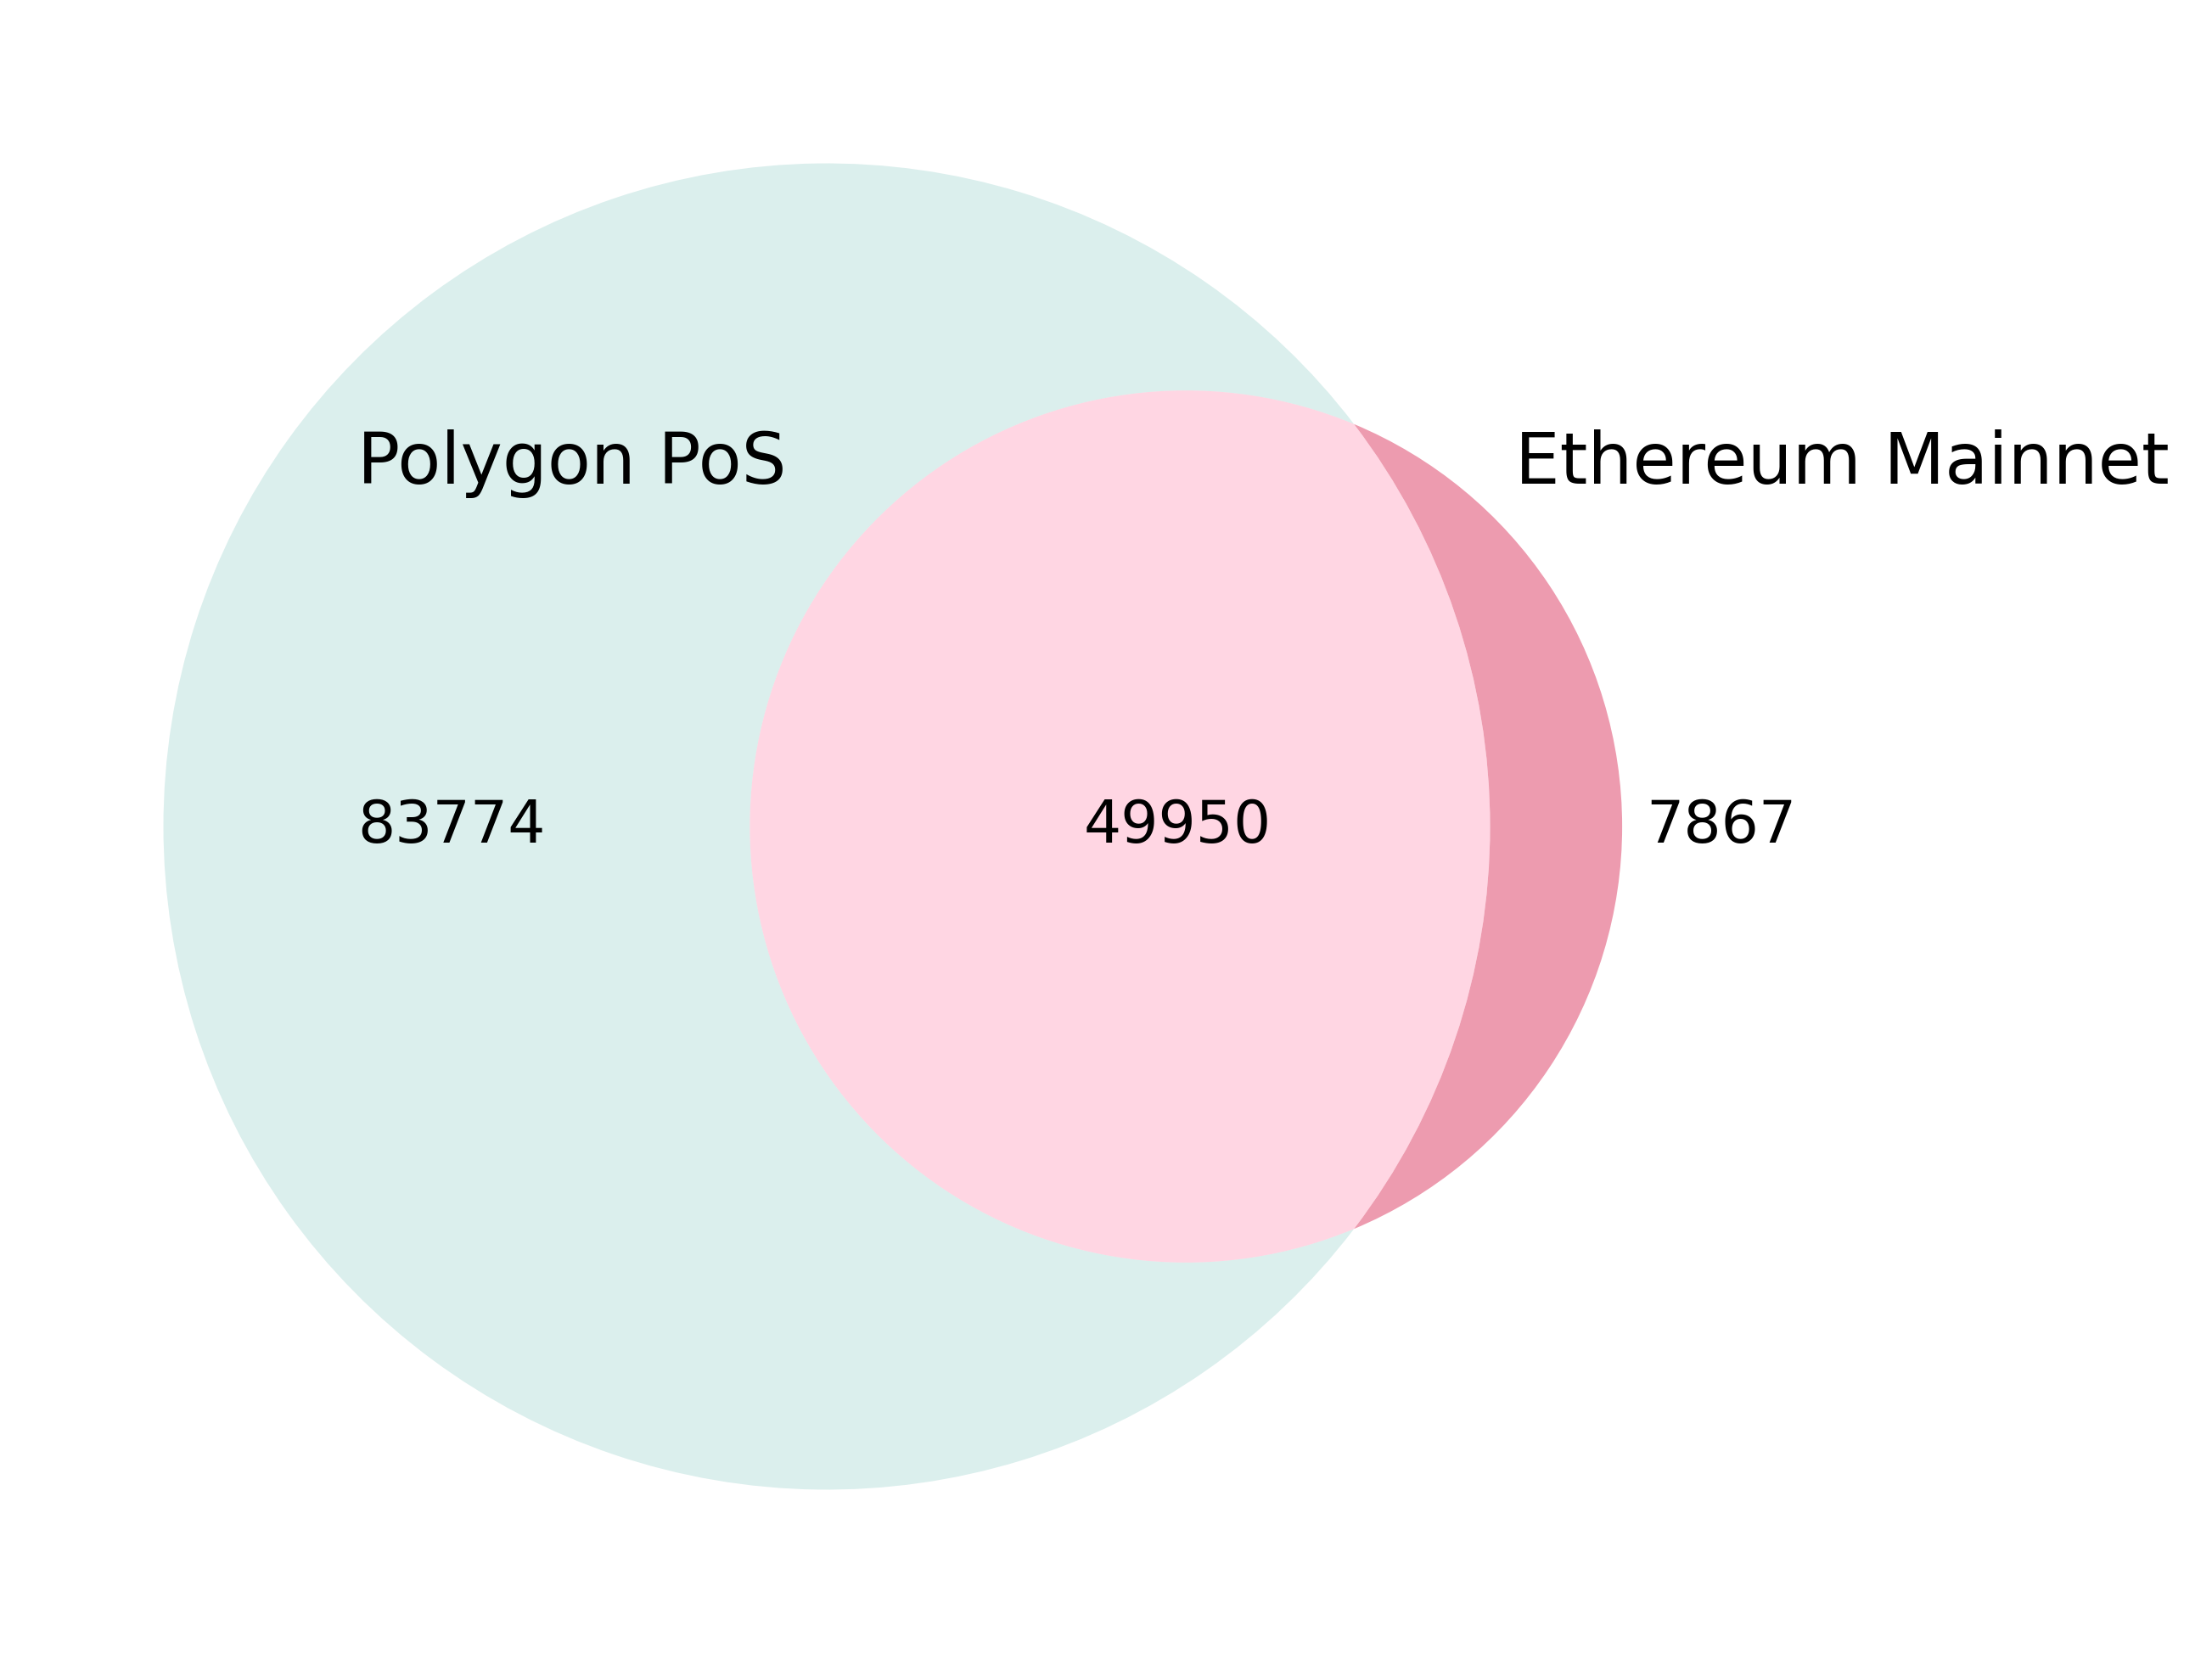
\includegraphics[width=0.6\textwidth]{../figures/venn_diagram.png}
	\caption{Address Subsets Visualized in a Venn Diagram}
	\label{fig:Venn}
\end{figure} 

\subsection{Transactions and Token Transfer Events}
The address subsets were used to collect transaction and token transfer event data from Ethereum and Polygon. Ethereum or Polygon data can be accessed directly through a node or an application programming interface (API) provider like Infura or Etherscan. The absence of account indexing in Ethereum or Polygon poses a challenge for retrieving all past transactions and token transfers of a specific address, as it requires scanning through all blocks and token transfer events emitted by designated token contracts. Fortunately, Etherscan offers an API Endpoint Module for ``Accounts`` that facilitates the retrieval of transactions and token transfer events for a given address. By using our network-specific address subsets, we were able to significantly decrease the number of required API calls. 
We gathered all transactions and token transfers up until block number \texttt{17,670,000} on Ethereum (July 11, 2023) and \texttt{44,990,000} on Polygon (July 12, 2023). In total, we collected over 30 million %30,689,978
token transfer events and more than 16 million %16,092,531
 normal transactions. While the amount of transactions is similar between the two networks, Polygon has roughly three times more transfer events. \newline The output was stored in separate CSV files and also imported into a MongoDB\footnote{\url{https://www.mongodb.com/}} database. The database contains distinct collections for transactions and transfers. For additional information on the data fields of each collection, see Appendix \ref{sec:database}. 

\iffalse
%Transfer Events: 30,689,978
%Transfer Events Ethereum: 7,832,778
%Transfer Events Polygon: 22,857,200
%Transactions = 16,092,531
%Transactions Ethereum = 8,448,584
%Transactions Polygon = 7,643,947
Figure X visualizes the number of daily transactions and token transfers for each chain.
\begin{figure}[h!]
	\centering
	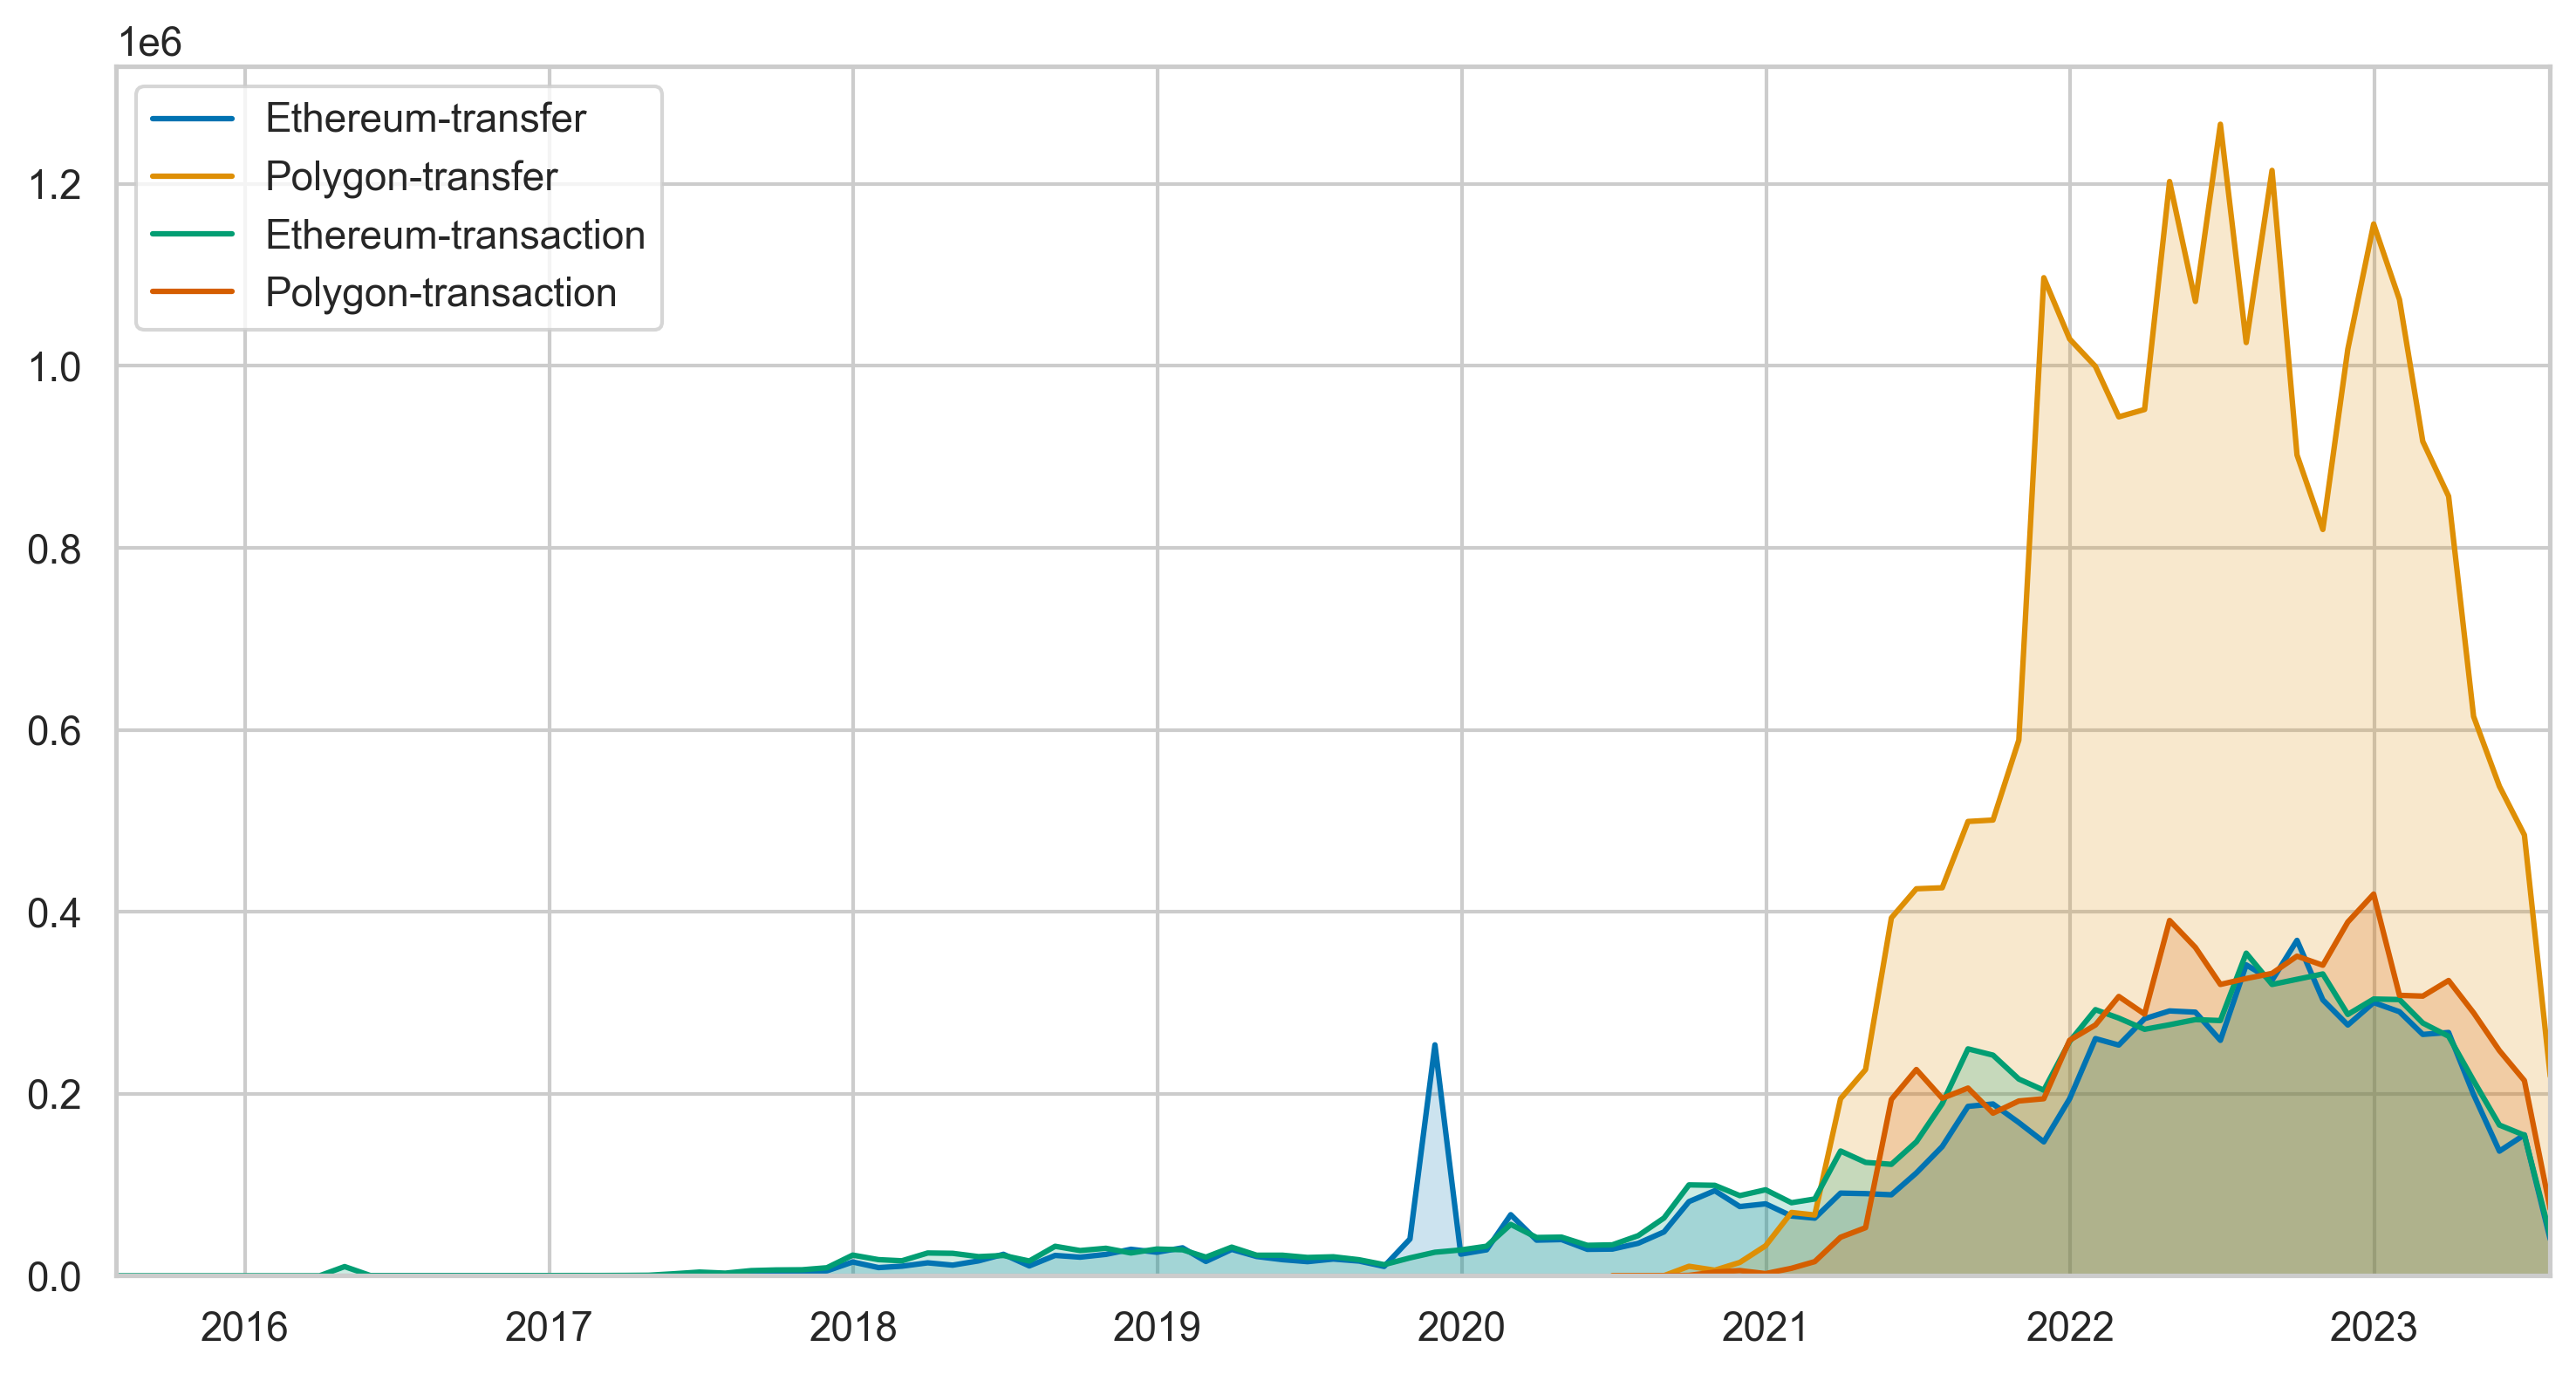
\includegraphics[width=\textwidth]{../figures/transfers_tx_by_chain.png}
	\caption{Monthly Transactions and Token Transfers by chain}
	\label{fig:Data}
\end{figure} 
\fi

\subsection{Intra-set asset transfers}
\label{sec:intra-set}
We want to employ entity clustering heuristics to determine the number of entities represented by the remaining 137,544 addresses. Or, to phrase it differently, do users interact with Decentraland using multiple EOAs, and can we identify addresses that belong to the same user?
\newline
To achieve this, we often only consider transactions or token transfer events where both the ``\texttt{from}`` (sender) and the ``\texttt{to}`` (recipient) address are within the address set. We call this reduced data set ``intra-set asset transfers``. Regarding normal transactions, this means that we only keep native asset transfers (payments), as almost all addresses are EOAs. \newline
The intra-set asset transfer data set is mainly used to generate the network graphs (see Section \ref{sec:node}).
When clustering addresses using graph-based approaches, this has the advantage that we do not need to differentiate between EOA and smart contract account later on. Furthermore, it allows us to observe and visualize the asset flows between users. In total, we have 974,478 intra-set token transfers and 210,548 intra-set native asset transfers/payments (101,621 Matic, 108,927 Ether). 

%(logging in to Decentraland with multiple addresses) When it comes to entity clustering, we essentially want to answer the question of how many real-world entities our remaining  137,544 addresses represent. 
%filter our transactions and token transfers to entries where both the 'from' and the 'to' are within this narrowed pool of addresses. We define this as intra-set asset transfers. For the transactions, this means that we only consider native asset (Ether or matic) transfers. %between two EOAs
%we focus on on-chain data (and not user location or avatar data), allowing us to exclude addresses that have not transacted or interacted with any token on Ethereum or Polygon. 
%As mentioned in the introduction, the goal of this paper is to cluster addresses belongig to the same entity that were recorded/active in Decentraland during the 9-month period. Therefore, we disregard addresses outside of this set. Also, since we only look at on-chain data, we cannot cluster addresses without activity on Polygon or Ethereum. Doing these two reductions, there are  141, 591 'clusterable' addresses remaining.
%Since all of our addresses are EOAs (some multisig smart contract wallets). 

\subsection{ENS address pairs}
\label{sec:ens}
Similarly to \cite{Beres2020}, we use Ethereum Name Service (ENS) identifiers as ground truth information to evaluate some of the clustering methods.\newline
\textit{ENS} is a naming system that relies on the Ethereum smart contracts. Its main purpose is to map human-readable names, such as \texttt{`alice.eth`}, to machine-readable identifiers, mostly Ethereum addresses. The architecture of ENS comprises two main components: the registry and resolvers. \newline
The \textit{ENS registry} consists of a single smart contract\footnote{The registry contract is ERC-721 compliant, which means that .eth registrations can be transferred in the same way as other NFTs.} that maintains a list of all domains and subdomains, recording the ``owner`` and ``resolver`` for each. The registry allows the owner of a domain to make changes to that data. \citep{ENSdocs} %Domain owners may set the resolver for the domain.
\newline
\textit{Resolvers} are responsible for %(the actual process of)
 translating names into addresses. Any contract that adheres to the relevant standards may act as a resolver. The process of resolving a name involves two steps: \textit{First}, the registry must be queried to find out which resolver is responsible for the name, and \textit{second}, that resolver must be asked for the response to the query. \newline
In addition to regular resolution from name to address, ENS also supports ``reverse resolution``, allowing for a mapping from address back to a name (or other metadata). Reverse resolution is accomplished via the %special
 domain \texttt{`addr.reverse`}% and the resolver function \texttt{name()}.
. This domain is owned by a special purpose registrar contract that allocates subdomains to the owner of the matching address - for instance, the address \texttt{`0x1234\dots`} may claim the name \texttt{`1234\dots.addr.reverse`}, and configure a resolver and records on it. The resolver in turn supports the \texttt{name()} function, which returns the ENS domain associated with that address.\newline
 Reverse resolution %(without a library)
 follows the same pattern as forward resolution: Get the resolver for \texttt{`1234....addr.reverse'} (where \texttt{`1234...`} is the address you want to reverse-resolve), and call the \texttt{name()} function on that resolver. However, ENS does not enforce the accuracy of reverse records. This means \texttt{`1234....addr.reverse`} may falsely claim that the name associated to their address is \texttt{`alice.eth`}. 
 
Figure \ref{fig:ENS} illustrates the mechanism that allowed us to generate ground truth pairs in a simplified way: Initially, the domain name \texttt{`foo.eth`} resolves to address \texttt{`0xABC...`}. The owner has also set a reverse resolution for this address, indicated by the the edge from the address to the domain name. Next, the owner decides to change the resolved address to \texttt{`0xDEF...`}, again setting a reverse record.  As a domain can only point to one address at the time, the previous mapping from \texttt{`foo.eth`} to the old address is deleted. However, \texttt{`ABC....addr.reverse`} still points to \texttt{`foo.eth`} and when we query the name corresponding to \texttt{`0xABC...`} and \texttt{`0xDEF...`}, both will return \texttt{`foo.eth`}.
If this special case occurs, we assume that both addresses belong to the same entity.
%We did not observe cases where someone set a reverse record to a completely unrelated address (e.g. alice.eth)

\begin{figure*}[h!]
	\begin{center}
		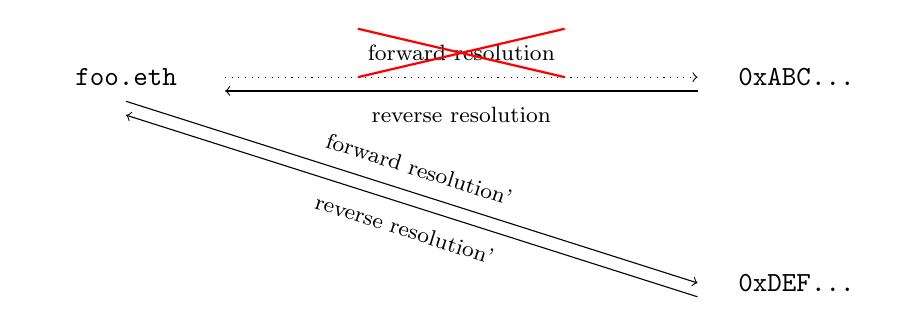
\begin{tikzpicture}[
    every node/.style={minimum width=2.5cm, minimum height=0.6cm, align=center},
    every path/.style={->},
    node distance=2cm and 6cm]

		\node (A) {\texttt{foo.eth}};
		\node[right=of A] (B) {\texttt{0xABC...}};
		\node[below=of B] (C) {\texttt{0xDEF...}};
		
		\draw[dotted] (A) -- (B) node[midway, above, name=pathAB] {\footnotesize{forward resolution}};
		\draw ([yshift=-5pt]B.west) -- ([yshift=-5pt]A.east) node[midway, below] {\footnotesize{reverse resolution}};
		\draw (A.south) -- (C.west) node[midway, sloped, above] {\footnotesize{forward resolution'}};
		\draw ([yshift=-5pt]C.west) -- ([yshift=-5pt]A.south) node[midway, sloped, below] {\footnotesize{reverse resolution'}}; 	
		
		% Adding a cross over "forward resolution"
        \draw[red, thick, -] (pathAB.south west) -- (pathAB.north east);
        \draw[red, thick, -] (pathAB.south east) -- (pathAB.north west);
							
		\end{tikzpicture}
		\caption{Changing the record to another address does not change the old reverse resolution (Simplified Schematic Representation)}
		\label{fig:ENS}
	\end{center}
\end{figure*}

We applied the following methodology to find ground truth pairs: \textit{First}, we gathered all addresses that interacted with ENS to reduce the amount of name look-ups. \textit{Second}, we iterated over each address and checked if it reverse-resolved to an ENS domain\footnote{This was done via the ENS module within web3.py \url{https://web3py.readthedocs.io/en/stable/ens_overview.html}, which provides an interface to look up domains and addresses.}. If so, we logged the ENS domain and address in a CSV file. \textit{Third}, using our new list, we identified if two addresses referenced the same ENS domain. If matched, we recorded both addresses alongside the ENS domain. \newline
From this, we identified 11,440 reverse records and 40 pairs of addresses pointing to the same ENS name, which we utilized as our ground truth to evaluate various clustering heuristics. Although this sample is relatively small, it allows us to assess and draw conclusions about the effectiveness of the methods.

%Check for each address in the list if the address points to an human-readable name. (reverse mapping must be set/configured) From the web3.py documentation \url{https://web3py.readthedocs.io/en/stable/ens_overview.html } %The ens module is included with web3.py. It provides an interface to look up domains and addresses, add resolver records, or get and set metadata.
%If two addresses point to the same ENS name we consider them belonging to the same entity. 
%Normally, one .eth domain cannot point/map to multiple Ethereum addresses. Forward resolution. This is likely due to the owner change and the record not updated.
%Only the forward resolution from the name to the address is changed. The reverse record resolution from the old address to the name is still there. For an visual explanation please see Figure \ref{fig:ENS}.
%Anyone who owns a domain at any level may configure subdomains - for themselves or others - as desired. For instance, if Alice owns 'alice.eth', she can create 'pay.alice.eth' and configure it as she wishes.
%Currently, all the subdomains or non .eth domains are not NFTs, unless the domain registrar itself supports NFT such as (dcl.eth, and .kred).
%If the owner sets a reverse resolution set with his new address, we have two addresses pointing to the same ens name. 
%While 'regular' resolution involves mapping from a name to an address, reverse resolution maps from an address back to a name - or other metadata. ENS supports reverse resolution to allow applications to display ENS names in place of hexadecimal addresses. Before this can be done, the owner of the address has to configure reverse resolution for their address.
%In spirit, it is similar to the well-known Domain Name Service (DNS). However, in ENS the registry is implemented in Ethereum smart contracts.
%Therefore, ENS provides a more user-friendly way of transferring assets on Ethereum, where users can use ENS names as recipient addresses instead of the error-prone hexadecimal Ethereum addresses.
%Resolving a name is a two-step process: First, ask the registry what resolver is responsible for the name, and second, ask that resolver for the answer to your query.\newline

%%%%%%%%%%%%%%%%%%%%%%%%%%%%%
%%% Clustering Heuristics %%%
%%%%%%%%%%%%%%%%%%%%%%%%%%%%%

\section{Clustering Heuristics}
In this section, we present an overview of clustering heuristics in the context of account-based blockchains and on-chain data. We will provide a detailed explanation of the mechanics and rationale behind the heuristic and assess its applicability to our case. 
In Section 5, we will implement and evaluate the heuristics we determine to be suitable for our objectives.

\subsection{Self-authorization} 
	All three token standards require functions to allow another address to transfer tokens on behalf of the actual owner. For the ERC-20 standard, this is achieved through the \texttt{`approve`} function, accepting the spender's address and the token amount as parameters\footnote{\texttt{approve(address spender, uint256 amount)}}. The ERC-721 has two functions dedicated to approvals: One for authorizing the transfer of a specific NFT\footnote{\texttt{approve(address to, uint256 tokenId)}} and one to permit transferring all of the owner's NFTs within the collection\footnote{\texttt{setApprovalForAll(address operator, bool approved)}}. The latter function also appears in the ERC-1155 standard. The approval functionality of these tokens is primarily used in connection with smart contracts (e.g., Decentralized Exchanges or NFT Marketplaces), but can also be applied for regular EOAs. \newline
The ``self authorization`` heuristic, proposed by \cite{FV:17}, suggests that users might authorize another address they own, possibly for risk distribution across several addresses or for testing purposes. \newline
Since all the addresses' transactions are available in our data set, we can easily employ this heuristic.

\iffalse
For the ERC-20 standard: \texttt{approve(address spender, uint256 amount)}
For the ERC-721 standard: \texttt{approve(address to, uint256 tokenId)} and \texttt{setApprovalForAll(address operator, bool approved)}\\
For the ERC-1155 standard: \texttt{setApprovalForAll(address operator, bool approved)}
\fi


\subsection{Deposit address reuse}
The concept of deposit address reuse was first introduced and systematically utilized by \cite{FV:17} and subsequently adoped by \cite{wu2022tutela}. This heuristic relies on the prevalent practice of crypto exchanges generating unique deposit addresses for each user. These addresses then forward the funds to an exchange's main address. It is highly likely that multiple addresses sending funds to the same deposit address are controlled by the same entity. The key challenge of this approach lies in identifying these deposit addresses, which could either be EOAs or smart contracts. \citep{FV:17}\newline
Deposit addresses share the characteristic that they forward the received funds to a major exchange account. Two parameters are essential for deposit address detection: the discrepancy between the amount received and forwarded (since the exchange must pay gas fees), and the time lag between receiving and forwarding funds.
However, our data set only includes the direct transactions or token transfers associated with the addresses. The transactions between deposit and main exchange address are absent. Consequently, this clustering heuristic is not applicable %with our data
 and it would require significantly more effort for gathering the required data.

\subsection{Airdrop multi participation}
Airdrops are popular token distribution mechanisms, and recipients are mostly chosen based on past protocol activity. Probably the most well known example is Uniswap's UNI airdrop, where each address that interacted with the protocol until a specified cutoff date received a fixed amount of 400 UNI tokens\footnote{\url{https://blog.uniswap.org/uni}}. Especially in the early days of airdrops, these distribution mechanisms were not Sybil-resistant, leading to people creating multiple addresses in anticipation of an airdrop. However, \cite{FV:17} argues that managing the tokens on all of these addresses is impractical, which is why they are often aggregated into one address. He finds around 500 same-source, fixed amount token distribution events with at least 1,000 recipients while also taking into account the block difference between the individual aidrop token transfers. He defines multi-participation when two airdrop recipients forward their tokens to a single address. Since we do not have a whole view of the airdrop distribution events, we are not able to find them within our data. One possible approach would include manual selection of known airdrops. However, this process takes very long and is not guaranteed to cluster a lot of addresses, since most new airdrop events were made with some kind of sybil-resistance. Nevertheless, to test this approach we searched for addresses that forwarded the UNI airdrop to another address. We found eight such transfers, but none involved two addresses sending funds to a third address.

\subsection{Graph representation learning}
\label{sec:node}
According to \cite{Beres2020}, \textit{node embedding} methods form a class of graph representation learning\footnote{Sometimes also referred to as ``network representation learning``} methods that map graph nodes to vectors in a low-dimensional vector space. These methods aim to represent vertices with similar neighborhood structure by vectors that are close in the vector space. \newline
\cite{Beres2020} first introduced this approach on a Ethereum transaction graph for the purpose of entity identification to pair Ethereum addresses associated with Tornado cash deposits and withdrawals. Building on this, \cite{wu2022tutela} refined and expanded one particular node embedding algorithm to deanonymize Ethereum users at scale. \newline
The foundation for these node-embedding methods is an undirected graph where nodes are composed of distinct addresses, and an edge is placed between two nodes if there is a transaction between them. \newline
To construct the network graph, we use the intra-set asset transfers described in section \ref{sec:intra-set}. This approach differs from the methodologies adopted by \cite{Beres2020} and \cite{wu2022tutela}. On one hand, \cite{Beres2020} collected all transactions and token transfer events of their address set, but did not refine this data to only include intra-set asset transfers. On the other hand, \cite{wu2022tutela} do not operate on a specific address set, but use all Ethereum transactions to build the network graph, ignoring token transfer events. After comparing these two methodologies with ours, we determined that intra-set asset transfers were the most effective for clustering a pre-defined set of addresses. %using node-embedding methods.
\newline
Using the network graph, node embedding methods seek to learn a function that projects a node to a $d$-dimensional vector representation (also called feature vector). This is a way of simplifying the graph information by associating each node with a point in the Euclidean space. Various node embedding methods have been developed and applied to different domains. \citep{rozemberczki2020difftovec} \newline
The intuition behind node-embedding approaches is that addresses which interact with the same set of addresses within the network graph should be close in Euclidean distance. \cite{Beres2020} cites two main reasons for this. Firstly, users with multiple accounts often interact with the same addresses or services from most of them. Secondly, when users move funds between their personal addresses, they may unintentionally reveal their address clusters. \newline
\cite{karateclub} provide a variety of node embedding methods as a Python library\footnote{\url{https://github.com/benedekrozemberczki/karateclub}}. They categorize the methods into neighborhood (proximity) preserving and structural. \newline
We focus on the three methods that performed best in \cite{Beres2020} experiments: ``Diff2Vec`` \citep{rozemberczki2020difftovec}, ``Role2Vec`` \citep{ahmed2018roletovec}, and ``Deepwalk`` \citep{perozzi2014}. Diff2Vec and DeepWalk are both neighborhood preserving, while Role2Vec is a structural node embedding method. Although all of these methods utilize random walks to capture graph information, they differ in their approaches to leveraging these random walks for constructing Euclidean feature vectors. A detailed explanation of each method is beyond the scope of this thesis. The interested reader may consult the originial publications. For a concise overview of Diff2Vec, please refer to \cite{wu2022tutela}. \newline
With our intra-set asset transfer data (\ref{sec:intra-set}) and ENS address pairs (\ref{sec:ens}), we were able to apply and evaluate the node embedding methods described above. Using the library described by \cite{karateclub} requires certain preprocessing steps for the network graph. Transactions must be treated as undirected edges and loops (self-transactions) and multi-edges should be removed. Moreover, nodes outside the largest connected component are excluded. The resulting network graph includes 51,566 nodes and 249,302 edges. \newline
It is worth noting that unlike \cite{wu2022tutela}, we decided not to include edge weights. For instance, if Alice sent Bob Ether three times and Bob sent Alice Ether two times, the edge weight would correspond to five. This choice facilitated the application of \cite{rozemberczki2020difftovec}'s library and eliminated the need to create a custom method. \newline
Based on our network graph, we generate 128-dimensional feature vectors for each address and method. \newline
Given an node embedding, we can search for the closest $k$ vectors to any given vector. As in \cite{wu2022tutela}, we accomplish this using FAISS (Facebook AI Similarity Search), developed by \cite{johnson2019faiss}, which always returns a list of $k$ nodes, ranked by their Euclidean distance to the given node\footnote{We set $k = 51566$, the total number of nodes in the network graph}. \newline
To evaluate the three node embedding algorithms, we use our ENS address pairs as ground truth. We run each node embedding method ten times and report the average rank of the target address. For comparison, we  compute the mean, median and standard deviation of the average rank for each method.

\iffalse
%write here that we tested different data sets to create the network graph but intra-set asset transfers performed best for our task.
The intuition of Diff2Vec is to summarize a node by its neighborhood through a diffusion-like random process. Specifically, there are four steps to Diff2Vec: 1) Generating a diffusion graph, 2) sampling a node sequence, 3) extracting features, 4) learning a neural network embedding
\fi

\subsection{Time-of-day transaction activity and gas price selection}
Apart from the node embedding methods applied to Ethereum transaction graphs, \cite{Beres2020} suggest employing clustering heuristics based on time-of-day transaction activity and gas price selection patterns. \newline
\textit{Time-of-day transaction activity} considers all transaction timestamps initiated by a particular address. These UNIX timestamps are transformed into hour-of-the-day-based values. The authors argue that account owners may expose daily activity patterns and represent addresses by a vector including the mean, median and standard deviation, as well as an activity histogram divided into four to six hour bins \citep{Beres2020}.  Figure \ref{fig:ToD} illustrates the time-of-day activity histogram and kernel density estimation (KDE) for a selected ENS address pair, divided into two hour intervals.\newline
Additionaly, the \textit{gas price distribution} heuristic leverages the possibility of users revealing patterns when choosing their gas price. Prior to EIP-1559\footnote{\url{https://eips.ethereum.org/EIPS/eip-1559}}, users could set the gas price manually. In practice, most wallet user interfaces offered three levels of gas prices: slow, average, and fast. Selecting the the fast option would ensure almost immediate inclusion in the blockchain. To account for changes in Ethereum traffic volume, the gas price is normalized by the daily network average. The combination of gas price levels users select forms their personal gas price profile. An account is represented by a vector including the mean, median, and standard deviation and a normalized gas price histogram divided into 50 bins, which they determined to be optimal for clustering performance. \citep{Beres2020} \newline
We will not employ both methods due to their significantly poorer stand-alone performance compared to node embeddings. Nevertheless, we test a two-step approach: In the first step, we implement Diff2Vec to find the 10 nearest neighbors. In the second step, we order the remaining addresses by their Euclidean distance derived from the time-of-day and/or gas price feature vectors. We analyze the impact of this two-step approach on the average rank of a target address.

\begin{figure}[h!]
	\centering
	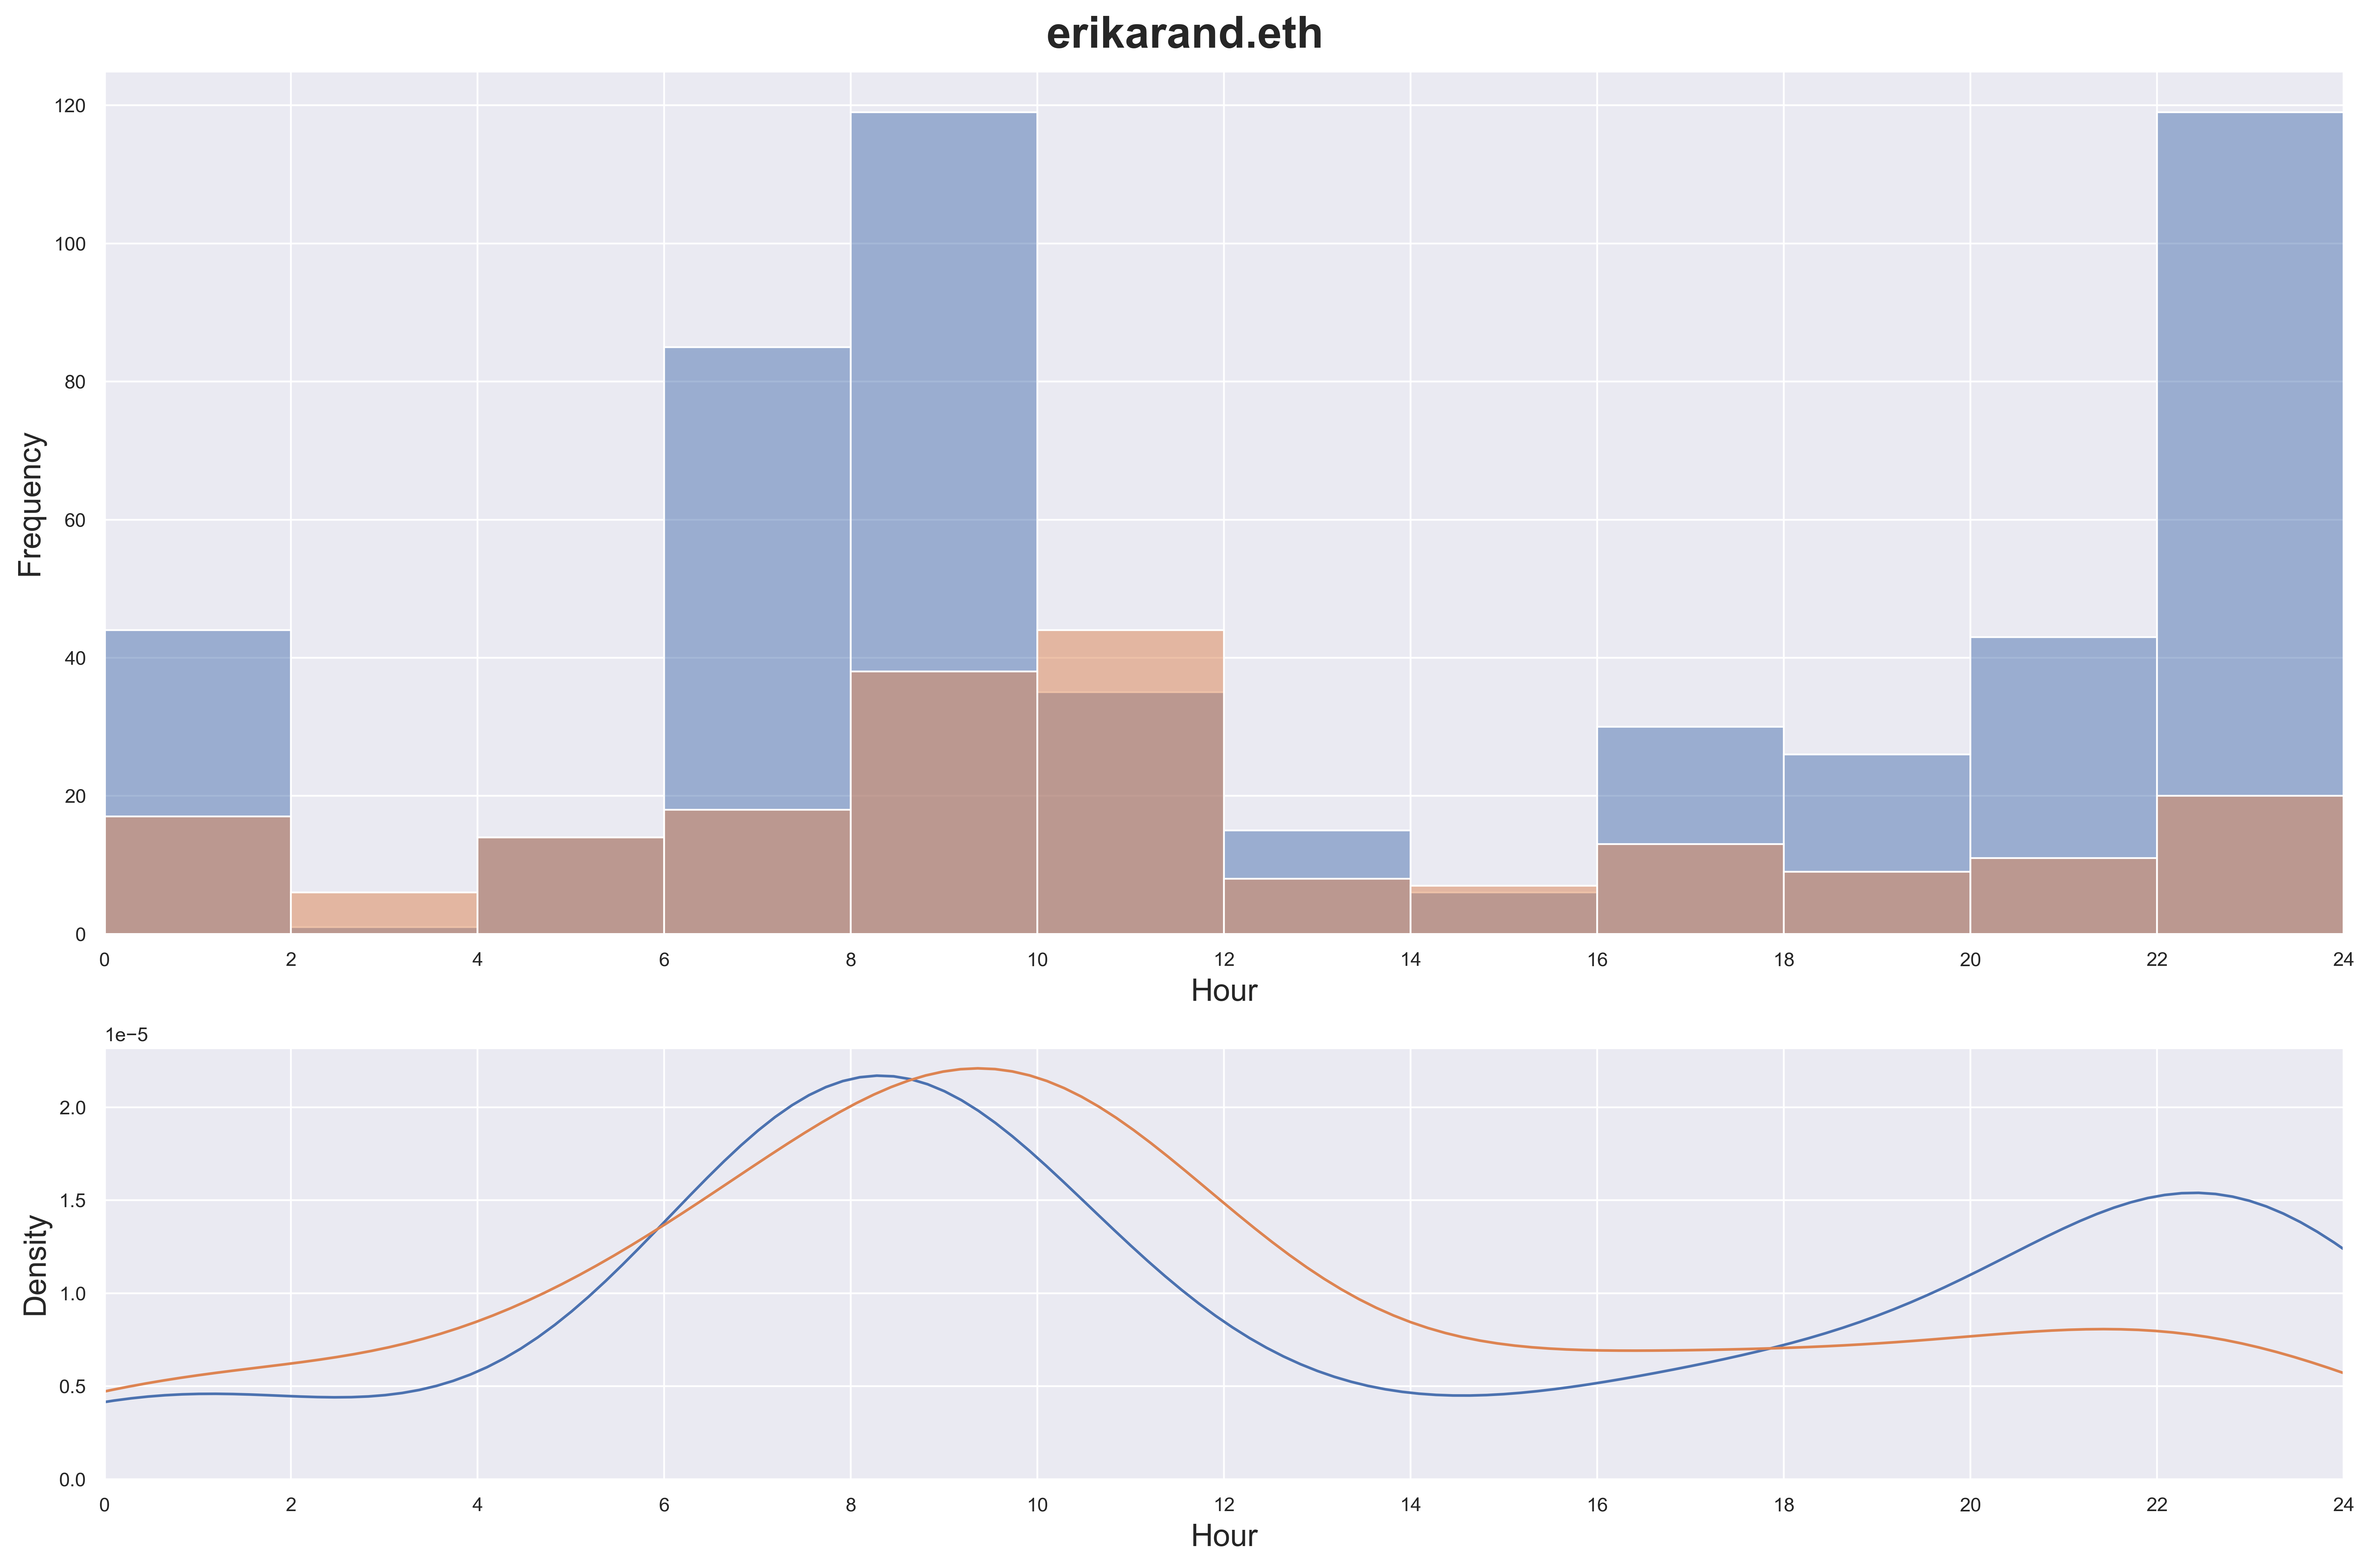
\includegraphics[width=0.8\textwidth]{../figures/time-of-day-activity.png}
	\caption{Time-of-day activity histogram and KDE for a selected ENS address pair}
	\label{fig:ToD}
\end{figure} 

\subsection{Tornado cash heuristics}
\cite{wu2022tutela} propose five heuristics targeted at Tornado cash, highlighting that careless user behavior can still reveal identity, despite using a mixer. The heuristics they identified are as follows: \newline
``Address match`` refers to instances where individuals use the same address for both depositing and withdrawing from the Tornado pool. ``Unique gas price`` involves users selecting a distinct gas price for both their deposit and withdrawal transactions (prior to EIP-1559). ``Linked ETH addresses`` examines whether a deposit address has interacted with a withdrawal address outside of Tornado Cash. ``Multiple denomination`` assesses an address' transaction history; two addresses with matching deposit and withdrawal portfolios are considered a pair. ``Torn minting`` identifies a specific user behavior when withdrawing so-called Anonymity points, an incentive scheme reward for increasing the anonymity set when depositing assets into Tornado cash.

We identified 84 transactions tied to Tornado cash pools, including 72 deposits, 10 withdrawals, and two transactions where an address sent 0.1 Ether to the corresponding pool without invoking the deposit function.  Despite applying all clustering heuristics except "Torn minting", we found no clusters.

\subsection{LAND transfers}
In addition to the existing clustering heuristics, we propose our own heuristic based on transfers of high-value NFTs such as LAND. We argue that, given the high value of Decentraland's land parcels, there is a strong likelihood that addresses are controlled by the same entity when LAND is transferred without any compensation. Users might perform such transfers to rearrange their LAND holdings, e.g., by upgrading to a more secure wallet. \newline
The primary challenge of this approach is to detect LAND transfers without any compensation. To accomplish this, we identify token or native asset transfers that took place within the same transaction as a LAND transfer. Upon manually examining various implementations of LAND trades on the most popular NFT marketplace contracts, we noticed a recurring pattern: the user address appears in both the ``from`` and ``to`` fields if a trade takes place. Figure \ref{fig:LAND_example} illustrates an example of this pattern. 
In the case of pure LAND transfers, the sending and receiving addresses are the same for all transfers within a transaction. However, this approach does not consider other LAND trading schemes, including off-chain compensation or non-atomic (within multiple transactions) trade settlement.

\begin{figure}[h!]
	\centering
	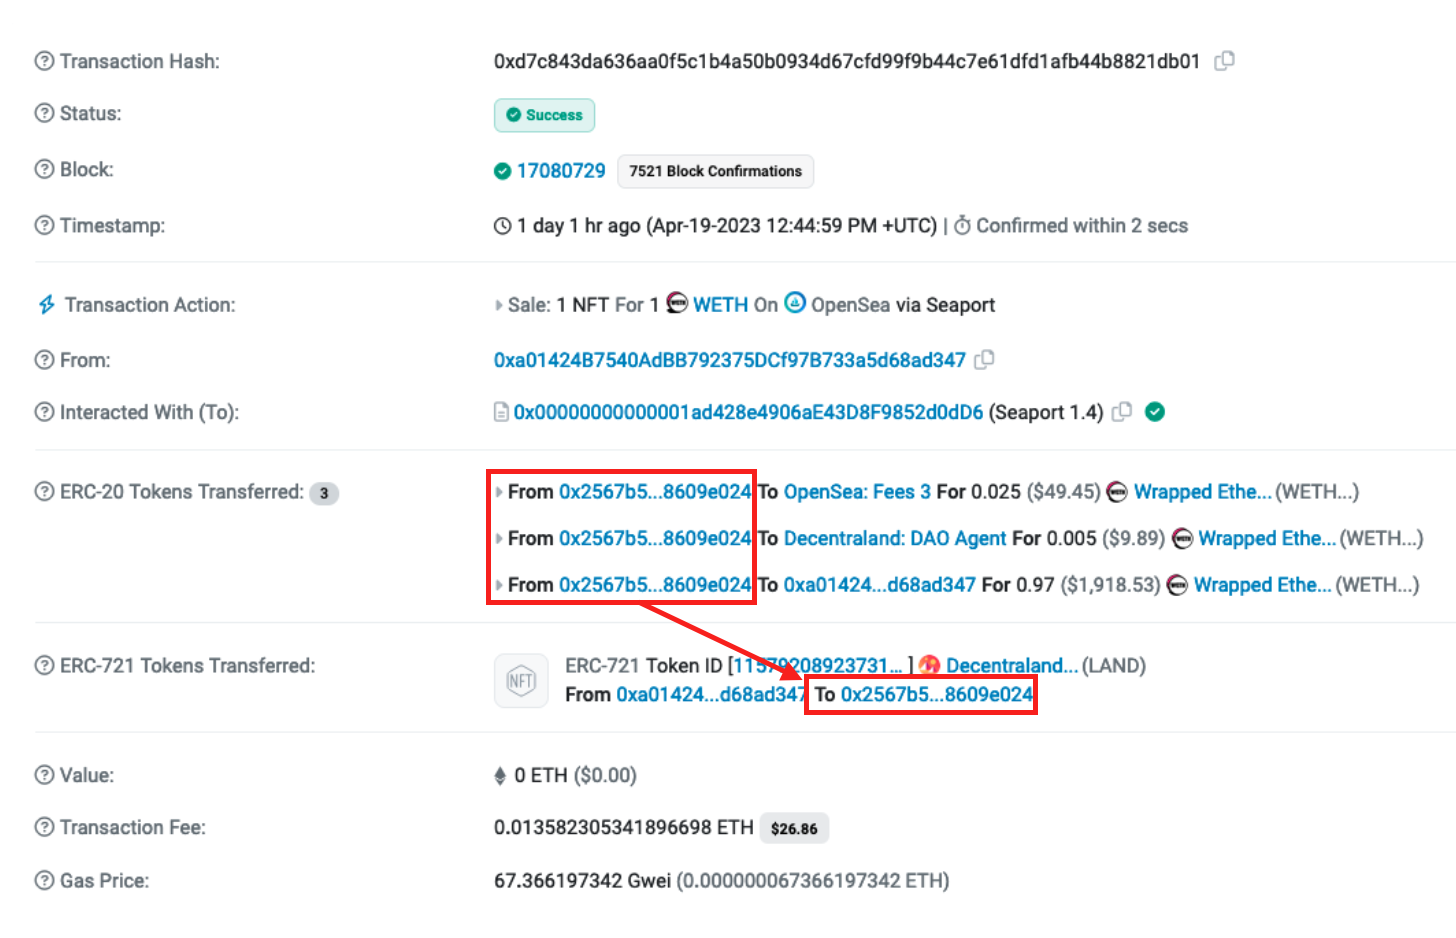
\includegraphics[width=\textwidth]{../figures/land-opensea.png}
	\caption{LAND trade on Opensea, Source: \href{https://etherscan.io/tx/0x2c2a70114e9080596bf5da6ad9c9b9f6d7e4c85a9d3b06e992f7248f9457a2ec}{Etherscan}}
	\label{fig:LAND_example}
\end{figure}

%%%%%%%%%%%%%%%%%%%%%
%%% Data Analysis %%%
%%%%%%%%%%%%%%%%%%%%%

\section{Data Analysis}
This section analyzes clustering heuristics applicable to our address set using the collected data. These include self-authorization, node embedding, and our proposed approach involving LAND transfers. %we describe our approach/method and the results.

\subsection{Self-authorization}
We analyze the addresses' transaction data to find self-authorizations, focusing on the transaction's ``calldata``. The first four bytes of the calldata represent the function selector, which unambiguously specifies the smart contract function the transaction originator wants to invoke. \newline
\textit{First}, we identify all transactions that begin with a function signature related to the approval functions corresponding to ERC-20, ERC-721, and ERC-1155 token standards. \textit{Second}, we extract the approved (spender) address, which is always located at the same position within the calldata due to token standardization. We then record the spender address in a new field within our dataframe. \textit{Third}, we implement two filters on the approval transactions. The first filter checks if the spender address is part of our address set, and the second ensures that the spender address is different from the address initiating the transaction, which may occur due to a user interface bug or testing transactions. \textit{Fourth}, we group the remaining approvals by the initiating address and form the clusters.

We identified 16 clusters across 126 self-authorizing transactions, comprising 115 distinct addresses. After manual inspection, we excluded a cluster containing 80 addresses with all approvals issued by the same address for the same token contract. The token contract represents a collection of wearable NFTs on Polygon called ``Renaissance King by René Mäkelä`` and may use an uncommon or potentially even faulty token minting scheme. Ultimately, we discovered 35 addresses associated with 15 distinct entities.

\subsection{Node embeddings}
Our analysis of node embedding methods starts with a network graph built from intra-set asset transfers. We treat addresses as nodes and add undirected edges between them if they interacted with each other. \newline
To use the Python library developed by \cite{karateclub}, we remove multi-edges and loops (transfers with the same sender and recipient address) and only consider nodes within the largest connected component. The resulting network graph includes 51,566 nodes and 249,302 edges. As previously stated, we utilize the Diff2Vec, Role2Vec, and DeepWalk methods from the library. \newline
Subsequently, we run ten independent experiments for each method. Our choice of input parameters is identical to \cite{Beres2020}. Each experiment returns a node embedding in the form of a matrix with 51,566 rows corresponding to the number of nodes in the graph, and 128 columns, representing the feature vector dimensions. \newline
For any node within the embedding, we can easily order all other nodes by the Euclidean distance. We achieve this through the FAISS Python library, which is suitable for efficient similarity search and clustering of dense vectors \citep{johnson2019faiss}.\newline 
This enables us to search for our ENS ground truth pairs and report their relative rank. The results for each address pair, averaged over ten experiments, are presented in Table \ref{tbl:ENS_Domain_Ranks}. Additionally, we calculated the mean, median, standard deviation, and the rate of the target address appearing within the five or ten nearest neighbors for each method.

All three methods demonstrated remarkable efficacy in locating the target address, which indicates their ability to find multiple addresses controlled by a single entity.
Role2Vec is the most effective method, with the target address, on average, found within the 28 nearest neighbors. In contrast, Diff2Vec and DeepWalk produced slightly higher averages of 46 and 62, respectively. Furthermore, Role2Vec found the target address within the ten nearest neighbors in 24 out of 34 cases (71\%). Diff2Vec is barely less effective than Role2Vec or DeepWalk, although still generally successful. \newline
Notably, two address pairs are not present within the network graph and therefore display no values. However, they have been included to demonstrate that the intra-set asset transfer approach may only sometimes be applicable to cluster all addresses of a predefined set. \newline
We also need to consider that average rank may not be the most appropriate evaluation metric, particularly when a user controls more than two addresses. Suppose a single entity controlling 20 addresses, but only one pair of addresses is detected as ground truth. Even if the algorithm finds all 20 addresses within the nearest neighbors but identifies the ground truth pair as the last one, we will score it lower than another algorithm that finds only one of the twenty addresses but within the ten nearest neighbors.

\begin{table}[h!]
\scriptsize
  \centering
  \begin{tabular}{lrrr}
    \hline
	\textbf{ENS domain name} & \textbf{Diff2Vec} & \textbf{Role2Vec} & \textbf{DeepWalk} \\
	\hline
	anisofim.eth & 2.5 & 6.2 & 2.7 \\
	arisalzberg.eth & 577.3 & 33.3 & 58.8 \\
	atearnz.eth & 2.8 & 2.5 & 3.3 \\
	awedjob.eth & 106.8 & 71.1 & 20.1 \\
	captvicky.eth & - & - & - \\
	disruptor.eth & 11.1 & 3.0 & 1.4 \\
	dragonkiller.eth & 30.7 & 1.0 & 1.0 \\
	eibriel.eth & 44.3 & 91.2 & 545.4 \\
	epdrabbit.eth & 16.3 & 10.4 & 4.1 \\
	erikarand.eth & 1.0 & 1.0 & 1.0 \\
	hyperspek.eth & 129.1 & 10.0 & 605.4 \\
	jamesmillerblog.eth & - & - & - \\
	jasonhsu.eth & 1.0 & 1.0 & 1.8 \\
	joeyz.eth & 1.9 & 1.0 & 1.0 \\
	keastie.eth & 10.4 & 1.0 & 18.2 \\
	linkg.eth & 4.0 & 1.0 & 10.3 \\
	lulox.eth & 4.2 & 1.5 & 27.2 \\
	maruudn.eth & 5.7 & 5.6 & 108.5 \\
	maryana.eth & 52.3 & 373.8 & 9.0 \\
	meanboss.eth & 9.0 & 9.0 & 51.8 \\
	metatiger.dcl.eth & 474.2 & 86.7 & 2.4 \\
	mgdivingnz.eth & 1.7 & 5.0 & 1.0 \\
	mrcryp.eth & 2.7 & 1.0 & 2.3 \\
	nicebhaiya.eth & 1.3 & 3.4 & 2.4 \\
	niceguy.eth & 1.0 & 1.0 & 2.2 \\
	ornellaweb3.eth & 3.7 & 2.0 & 284.0 \\
	pinkboots.eth & 16.9 & 14.4 & 2.2 \\
	remx.eth & 3.6 & 2.6 & 1.7 \\
	rileybeans.eth & 1.5 & 2.0 & 1.6 \\
	robertjames.eth & 2.7 & 1.0 & 1.1 \\
	rsantos.eth & 2.0 & 13.6 & 101.2 \\
	sannin.eth & 64.8 & 1.1 & 1.6 \\
	smileface.eth & 3.0 & 19.3 & 1.7 \\
	theartcollection.eth & 11.0 & 5.6 & 3.4 \\
	turkii13.eth & 52.1 & 68.9 & 47.3 \\
	tweetious.eth & 10.3 & 4.0 & 227.0 \\
    \hline
    Mean & 46.038 & 28.073 & 62.084 \\
    Median & 4.2 & 3.4 & 3.3 \\
    Standard deviation & 120.504 & 68.814 &  139.932\\
    Within 5 nearest neighbors & 17 (0.5) & 19 (0.56) & 20 (0.59) \\
    Within 10 nearest neighbors & 19 (0.56) & 24 (0.71) & 21 (0.62)\\
    \hline
  \end{tabular}
  \caption{Average Rank of ENS Domain Names for Different Embedding Methods}
  \label{tbl:ENS_Domain_Ranks}
\end{table}

After evaluating the different node embedding methods, we want to cluster the addresses to assess the number of entities represented by the 51,566 nodes in the network. We use the node embedding generated by Role2Vec. \newline
One approach might involve grouping a node's $k$ nearest neighbours to a cluster and subsequently merging clusters until each node is assigned to exactly one cluster. However, selecting an appropriate $k$ is challenging, and it is hard to make the case that each address belongs to a cluster of at least $k$. \newline
Instead, we choose to build clusters based on the Euclidean distance. All neighbors of a node below a certain threshold are considered a cluster. Afterward, we merge overlapping clusters; for instance, if node A is clustered with nodes B and C, and node C is clustered with nodes A and X, we form a cluster comprising A, B, C, and X. \newline
We explore the sensitivity of clusters to various Euclidean distance threshold values. Figure \ref{fig:threshold_sensitivity} shows the histogram of cluster sizes and Table \ref{tbl:cluster_table} displays the number of resulting clusters depending on various threshold values. We chose said values after observing the distance between ground truth pairs. For better visibility, we only display clusters below 20 addresses in Figure \ref{fig:threshold_sensitivity}. At thresholds of 0.6, 0.7, and 0.8, we find 23,608, 18,592, and 14,793 clusters, respectively. Regardless of the threshold, the largest cluster has more than 500 addresses. Unsurprisingly, higher thresholds result in fewer single-address clusters and more large sized clusters. The effect of the threshold is most pronounced for single address clusters, while affecting other cluster sizes much less. 

\begin{figure}[h]
	\centering
	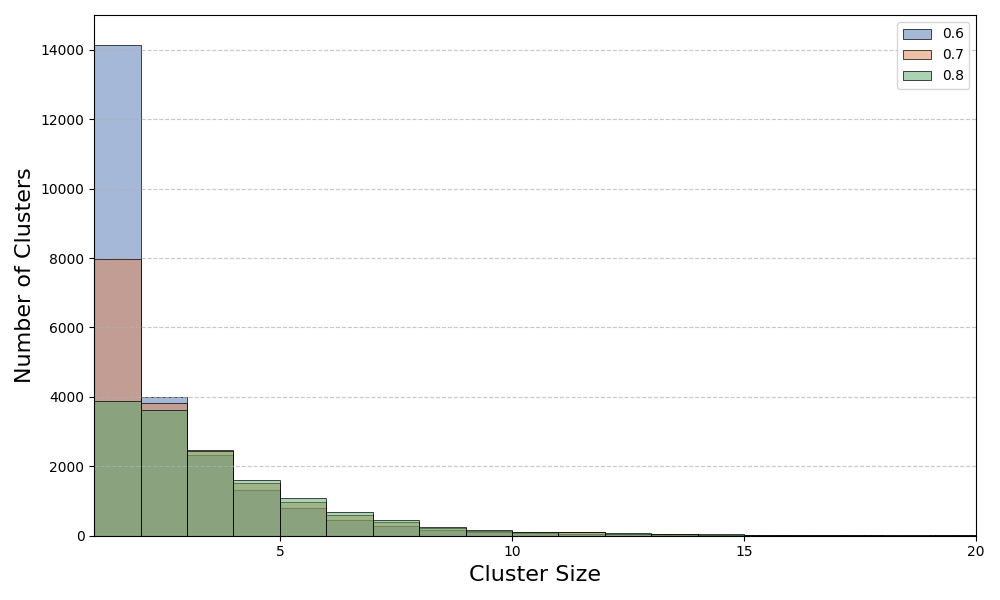
\includegraphics[width=\textwidth]{../figures/cluster_histogram.png}
	\caption{Cluster Size Histogram for different distance thresholds}
	\label{fig:threshold_sensitivity}
\end{figure}


\begin{table}[h!]
\scriptsize
  \centering
  \begin{tabular}{lrrrrrrr}
    \hline
	\textbf{Threshold} & \textbf{0.5} & \textbf{0.55} &\textbf{0.6} & \textbf{0.65} & \textbf{0.7} & \textbf{0.75} & \textbf{0.8} \\
	\hline
Total clusters 			& 29,502 & 26,762 & 23,608 & 21,229 & 18,592 & 16,361 & 14,793 \\
Size of largest cluster & 499 & 	512 & 516 & 	524 & 532 & 535 & 544\\
Clusters of size 50+ 	& 2 & 2 & 3 & 7 & 9  & 13 & 14\\
    \hline
  \end{tabular}
  \caption{Clustering results for different threshold values}
  \label{tbl:cluster_table}
\end{table}

\subsection{LAND transfers}
To implement the LAND transfer clustering heuristic, we select all transaction hashes of LAND transfers between two Decentraland addresses. Next, we gather all token and native asset transfers associated with the selected transaction hashes. We group the data by transaction hash and examine each transfer's sender (\texttt{from}) and recipient (\texttt{to}) address. If the same user address appears as the sender and recipient, we mark the transaction as a purchase. Finally, we filter out purchases and create address clusters based on the remaining LAND transfers.

A total of 740 LAND transfers were recorded, involving 413 unique addresses. Of these transfers, none involved any form of compensation within the same transaction. Upon analysis, we were able to group these addresses into 161 distinct clusters. The distribution of these clusters is shown in Figure \ref{fig:LAND_clusters}. Notably, the majority of clusters consist of two or three addresses. However, one cluster stands out, containing a significantly higher count of 71 addresses. This prominent cluster has been marked in green for ease of identification. \newline
LAND transfers between Decentraland addresses can also be visualized as a token network graph, as shown in Figure \ref{fig:LAND_network}. In this graph, red edges signify simple transfers, whereas blue edges represent LAND transfers made as part of a trade. Notably, the 71-address cluster previously mentioned is visible on the top-right of the largest connected component. \newline
A few key observations can be made from this network graph. In line with our expectations, most LAND transfers involve some form of compensation. Moreover, certain nodes play a central role in LAND trading, indicated by their high connectivity within the network. Lastly, a recurring behavior pattern is observed wherein an individual address purchases LAND and subsequently transfers it to a third address. %This could reflect a common strategy among participants in the LAND market.

\begin{figure}[h]
	\centering
	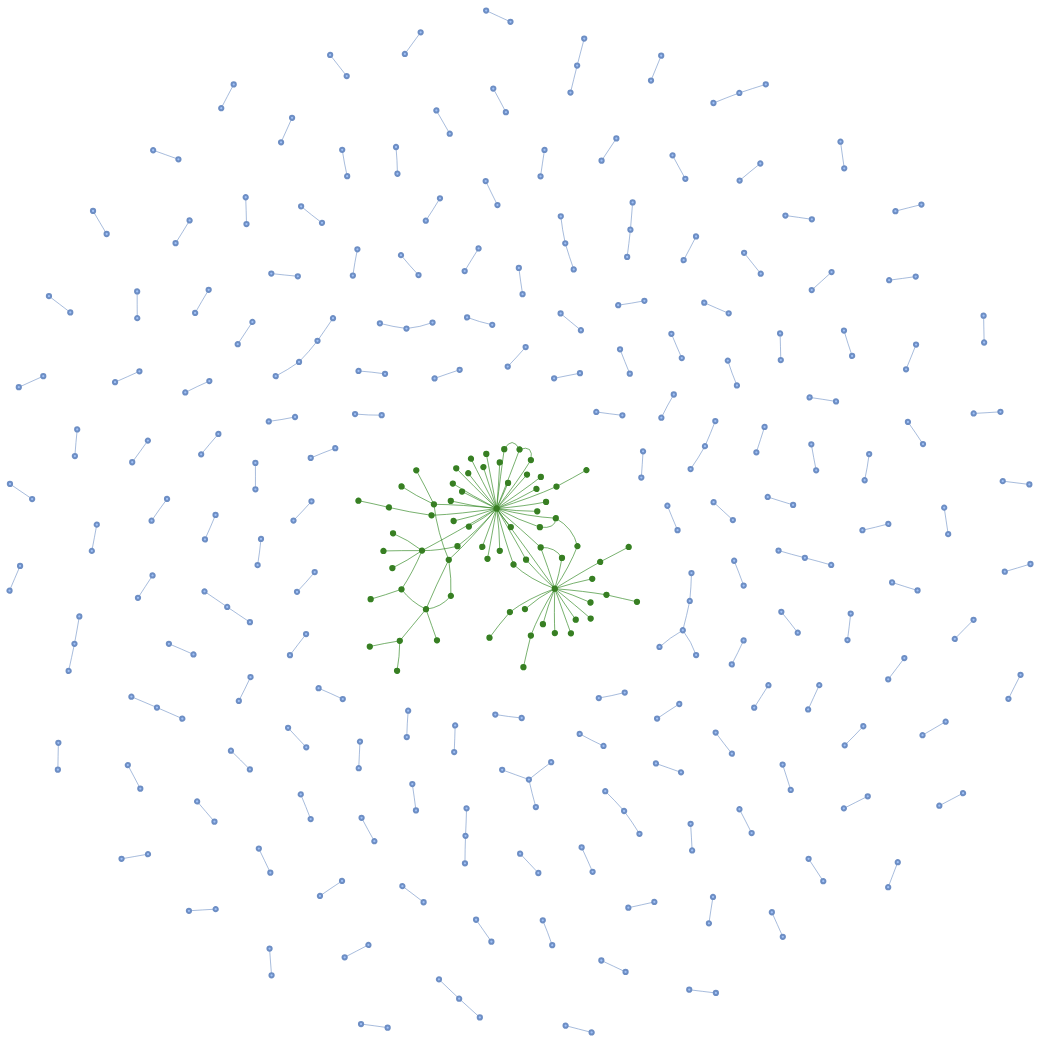
\includegraphics[width=0.5\textwidth]{../figures/land_clusters.png}
	\caption{Resulting LAND clusters, with largest cluster marked in green}
	\label{fig:LAND_clusters}
\end{figure}

\begin{figure}[h]
	\centering
	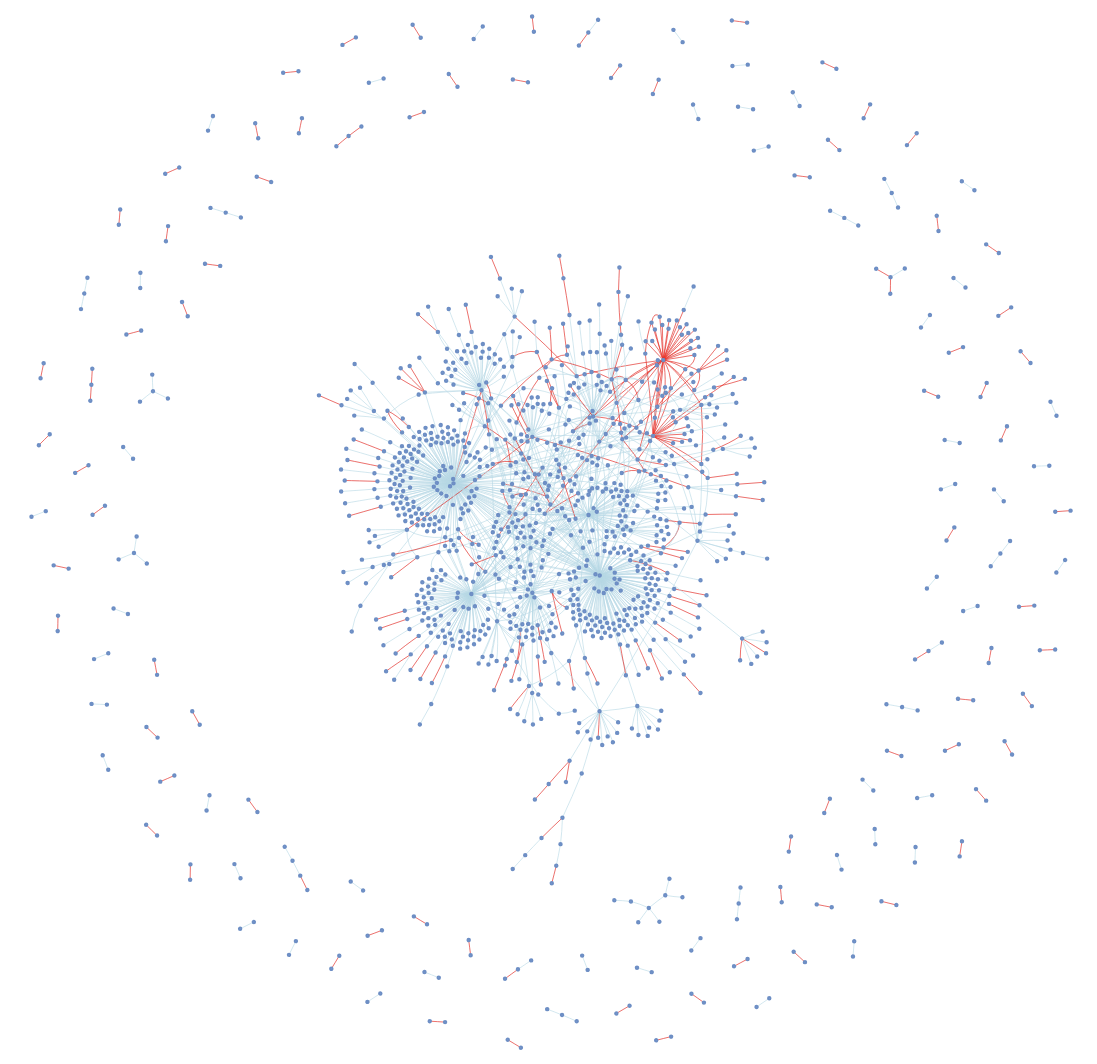
\includegraphics[width=\textwidth]{../figures/land_network.png}
	\caption{LAND token network}
	\label{fig:LAND_network}
\end{figure} 

\subsection{Combining clustering results}
To conclude our clustering analysis, we combine the results of self-authorization, learned node embedding and LAND transfer heuristics. By doing so, we can cluster 51,581 out of 137,544 (37.5\%) addresses that represent 29,680 entities. 
For the remaining addresses, we consider each as an individual entity. 
We applied a strict distance threshold of 0.5 for clustering embeddings generated by Role2Vec and excluded the 80-address cluster identified in self-authorization.
Under these assumptions, we estimate 115,643 active users during the time frame studied. Out of these, 8,483 entities (7.3\%) interacted with Decentraland through multiple addresses. The largest entity comprises 499 addresses. We plot the distribution of cluster sizes in Figure \ref{fig:barplot_clusters}.

\begin{figure}[h]
	\centering
	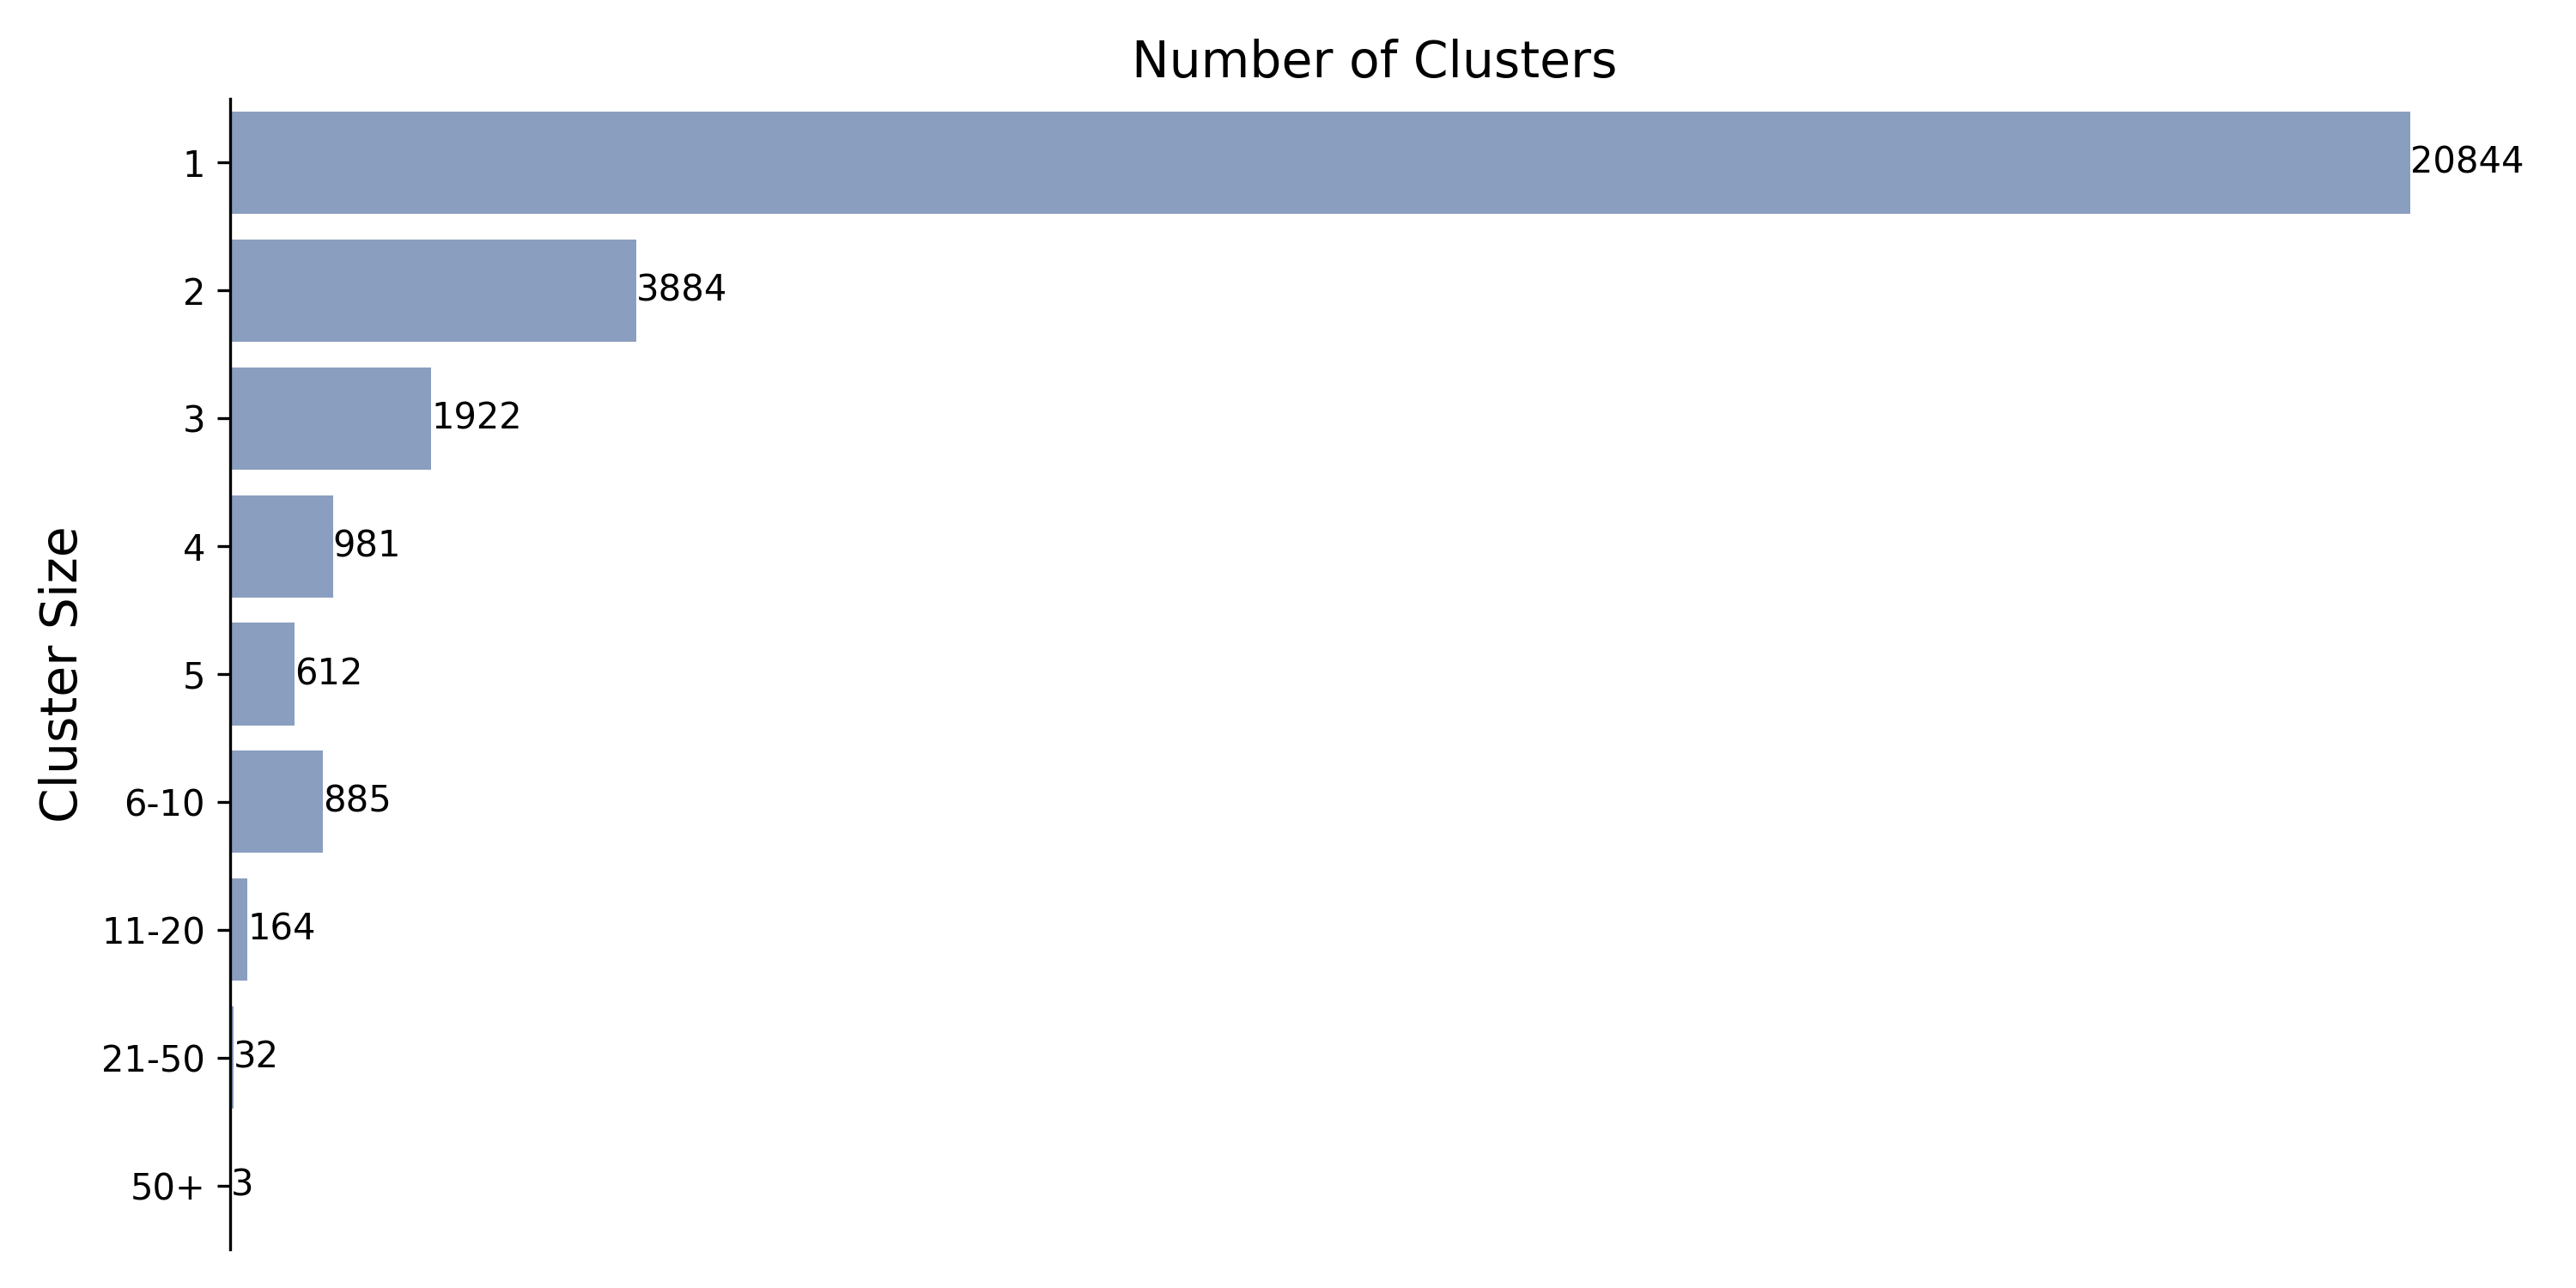
\includegraphics[width=\textwidth]{../figures/cluster-size-distribution.png}
	\caption{Number of clusters by Cluster Size}
	\label{fig:barplot_clusters}
\end{figure}


%%%%%%%%%%%%%%%%%%
%%% Discussion %%%
%%%%%%%%%%%%%%%%%%

\section{Discussion}

%The results chapter or section simply and objectively reports what you found, without speculating on why you found these results. 
%The discussion
%... interprets the meaning of the results, puts them in context, and explains why they matter.
%... is an in-depth exploration of the results, going into detail about the meaning of your findings and citing relevant sources to put them in context.
%... Try to explain "What do your results mean?", and how they relate to the literature,
%... provides the explanation and interpretation of results or findings by comparing with the findings in prior studies.

Throughout our analysis, we successfully applied three heuristics to cluster our address set while making use of on-chain data. In the following discussion, we will examine each of the approaches step-by-step.

Implementing the \textit{self-authorization} heuristic is straightforward, but results in very few identified address clusters. This is because it requires a highly specific on-chain behavior, which is rarely observed in practice. In particular, approvals are seldom used to authorize another externally owned account one might own. We also encountered a significant number of false-positives due to non-standard implementations. We are very confident that the large cluster is not controlled by the same entity, and therefore remove it. After excluding these instances, we identified a total of 15 entities consisting of 35 addresses. This outcome aligns with findings by \cite{FV:17}, who also observed that the heuristic captures only a small proportion of addresses. In his analysis of Ethereum transaction data up to block number 8,500,000 he identified 4,599 entities from 7,107 addresses.

Address clustering through \textit{graph representation learning} proved to be the most effective approach in our analysis. Unlike methods that require participation in specific on-chain events, node embedding algorithms examine the entire asset transfer network between addresses, making it broadly applicable. \newline
Our implementation of node embedding methods differs from previous approaches by \cite{Beres2020} and \cite{wu2022tutela}, the main reason being different settings and research questions. We construct the network graph based on asset transfers within our address set and simultaneously analyze Polygon and Ethereum data. \newline
Conversely, \cite{wu2022tutela} aim to cluster addresses without a predefined set, therefore using Ethereum transaction data for network graph construction. \cite{Beres2020} try to match deposit and withdrawal addresses for Tornado Cash, relying on all token transfers and transactions to cluster addresses based on similar on-chain behavior. Since it is not very common that Tornado cash withdrawal and deposit addresses interact with each other, the approach chosen by \cite{Beres2020} is better suited for their objectives. \newline
Moreover, we validated our approach and found better results in terms of average rank of ground truth address pairs, when building the network graph from intra-set asset transfers compared to using all token transfer events and/or transactions. A possible extension would include incorporating edge weights, similar to \cite{wu2022tutela}, however, we refrained from doing this because we would have needed to implement a custom node embedding algorithm.\newline
We applied three node embedding algorithms that delivered robust results in the experiments by \cite{Beres2020} and assessed their effectiveness in detecting ground truth pairs. Our results indicate that Role2Vec is the best-performing method, locating the ground truth pair within the five nearest neighbors in 70\% of cases.  This diverges from the findings of \cite{Beres2020}, who determined Diff2Vec to be the superior method among the three evaluated. \newline
Determining why one approach outperforms another is challenging. DeepWalk and Diff2Vec, both neighborhood-preserving algorithms, mainly capture node proximity. As noted by \cite{ahmed2018roletovec}, this does not necessarily imply similarity, especially when addresses frequently interact with each other without being controlled by the same entity. In contrast, Role2Vec, a structural node embedding method, identifies nodes with similar roles within the network. In our evaluation sample, network position or role may better represent similarity and structural relatedness among nodes. Despite these insights, the differences in results could be specific to the data at hand, given the small sample size, potential evaluation metric flaws, and the overall robust performance of all methods. \newline
Creating clusters out of the node embeddings, enables us to estimate the number of entities represented by the 51,566 addresses. Our method involves calculating the Euclidean distance between pairs of feature vectors, specifically using the node embedding matrix generated by Role2Vec. Nodes are clustered if their distance falls below a predetermined threshold, and any overlapping clusters are subsequently merged. \newline 
While our clustering method may not be ideal, it is probably more effective than clustering a fixed number of $k$ neighbors for each node. We observed that the number of clusters and their size is highly sensitive to the chosen distance threshold, making it challenging to assess the accuracy of these clusters. We have provided a sensitivity analysis to illustrate this issue. The distances between the feature vectors tend to be quite narrow, with significant variation even among various ground truth pairs' distances. Regardless of the threshold value, we were able to locate a cluster of more than 500 addresses. Manual inspection revealed that these address show very similar on-chain patterns: They are all exclusively active on Polygon and most of the transfers are mints of Decentraland related NFTs. Further, they transfer some NFTs to address \texttt{``0xE2e2F2240a84A61B7dFF50a86ee10d5FaF7faCa8``}. The transfers to and from this address are shown in Figure \ref{fig:cluster}. Incoming transfers are indicated by green edges, while outgoing transfers are shown by red edges. We hypothesize that the network in question may be operated by a user or even bot that creates multiple distinct addresses and actively engages with Decentraland. It seems likely that this bot may target specific locations or events where NFTs are (automatically) air-dropped to avatars in presence. If the NFTs hold value, the bot may then aggregate them to the main address and sell them on the Decentraland marketplace. This hypothesis could be verified with the Decentraland movement data. \newline
Notably, despite the limited on-chain data available, the node embedding algorithm was able to detect this activity pattern. Bot activity may become a concern for open and permissionless metaverse platforms like Decentraland and an interesting topic for future research. \newline
Finally, we explored potential enhancements to the graph representation learning method, such as incorporating time-of-day-activity and/or gas price selection information into the feature vectors generated by Role2Vec. Unfortunately, these modifications did not lead to any significant improvements. This outcome may be attributed to challenges in implementation, particularly in scaling the values without disturbing the integrity of the dense feature vectors.  
Similarly, a two-step approach for clustering, re-ranking the nearest neighbors of a node according to similarity in time-of-day activity and/or normalized gas price vectors, proved unsuccessful. These ideas remain open for further development of clustering heuristics in the future.

\begin{figure}[h!]
	\centering
	\includegraphics[width=0.65\textwidth]{../figures/network_visualization_0xe2e.png}
	\caption{Token Transfer Graph for \texttt{0xE2e2F$\dots$faCa8}}
	\label{fig:cluster}
\end{figure}

The \textit{LAND transfer} heuristic is targeted at users revealing address clusters by sending high-value assets to other addresses. In this specific case, we use the information that all addresses are related to Decentraland and therefore analyze LAND transfers. However, the approach could be applied (more generally) to other NFT collections or large asset transfers in general. \newline
The main assumption behind this approach is that users may want to reorganize their accounts from time to time, mostly to increase security guarantees or spread the risk across multiple accounts. As a concrete example, some users may have started with a simple browser-based wallet but as the value of their assets increased and their knowledge grew, they switched to a more secure hardware wallet. We detect 161 entities with 413 addresses applying this approach. One cluster with 70 address is very likely a not a single entity. It includes an address that participated in the intial LAND auction and subsequently distributed LAND. This may have happened through off-chain compensation. The advantage of this method is that it is relatively easy to visualise and understand. The disadvantage is that it demands a specific on-chain behaviour and is only scalable with significant effort. Additionally, many events that occur off-chain are not detectable in the data, resulting in an increased occurrence of false positives. 

Ultimately, we combined the results for each clustering heuristic mentioned above. Consequently, we managed to cluster 51,518 addresses, corresponding to 29,680 distinct entities. When adding the unclustered addresses, we identified 115,643 active users during the nine months, with 8,483 entities interacting through multiple addresses. \newline
These results, however, are heavily influenced by the assumptions we made. We were conservative by setting a low distance threshold and treating all other addresses as individual entities. Raising the threshold would result in larger clusters and fewer entities. \newline 
The majority of addresses were clustered through graph representation learning methods. Unlike other clustering heuristics, this approach does not rely on specific on-chain behavior patterns or participation in particular events. Our implementation generally captures all addresses that have transferred within the address set at least once. Nevertheless, some clusters may still go undetected, while others may overestimate the number of addresses within a cluster. It is important to note that these methods are still only heuristic and testing their efficacy on a large scale is not possible. \newline
Role2Vec performed best for our small test sample, but is not necessarily always be superior to Diff2Vec or DeepWalk. Incorporating time-of-day and normalized gas into feature vectors, or refining clusters using a two-step approach, requires further research but could enhance clustering results.

%%%%%%%%%%%%%%%%%%
%%% Conclusion %%%
%%%%%%%%%%%%%%%%%%

\section{Conclusion}

%...Re-state the main points in a new concise way that you want your readers to remember.
%...write the output of the work/ investigations in summarized form
%...intended to help the reader understand why your research should matter to them after they have finished reading the paper.
%...not merely a summary of your points or a re-statement of your research problem but a synthesis of key points. For most essays, one well-developed paragraph is sufficient for a conclusion, although in some cases, a two-or-three paragraph conclusion may be required.

The goal of this thesis was to identify the number of entities represented by the 473,927 addresses observed in Decentraland between July 16, 2022 and April 23, 2023. \newline
By exploiting activity patterns within the publicly available on-chain data, we are apble to apply various heuristics for clustering addresses controlled by the same entity. Focusing on Ethereum and Polygon on-chain data, we narrowed the address set down to 137,544.
After introducing various concepts needed to understand this complex topic, we efficiently collected the required on-chain data. This feat was achieved by using information if an address was active on Ethereum and Polygon and subsequently gathering all transactions and token transfers related to the addresses via Etherscan.

ENS pairs ...

We looked at the existing clustering heuristics and discussed their applicablilty to our research question/setting.
We found thee clustering heuristics, namely self-authorization, graph representation learning and non-compensated LAND transfers to be applicable to cluster a predefined address set. Self-authorization and graph representation learning through Ethereum transaction data were approaches proposed by \cite{FV:17} and \cite{Beres2020} respectively, while the LAND transfer heuristic was proposed by ourselves. We modified and extended the learned graph representation approach to best work with our research goal. As of our best knowledge, we are the first to work with intra-set asset transfers to construct the network graph for graph-representation learning.\newline 
The most successful clustering heuristic was graph representation learning, the reason being its general applicability, as it does not require participation in specific on-chain event / usage pattern. Topic for future research ... \newline
The node embedding approach could be possibly further extended by incorporating time-of-day activity or gas price selection patterns for better clustering performance of predefined address sets. \newline
Specifically looking at node embedding algorithms, we found the Role2Vec algorithm to be the most effective, finding the ground truth pair within the five nearest neighbors in 71 percent.

Results/ Evaluation ...

Clustering based on distance threshold, clusters dependent on this threshold...

Visualizations ...

Somethin about bots ...

Still a lot of natural activity on Decentraland and open infrastructure allows us to analyze it in detail as in this paper, exciting to analyze other things, endless possibilities.
Address clustering will  make further advancements. From a user perspective it is important that privacy enhancing protocols are also further developed and users educated how to preserve privacy when transacting on blockchains. / in the context of blockchains


%1. Public blockchain -> all data available -> allows us to analyse it and find information
%2. Clustering heuristics for account-based blockchains using on-chain data and on specific predefined address set
%3. sehr vielversprechend
%4. From the various methods Role2Vec best
%5. Summarize Final results
%6. For researchers -> extend this approach -> apply it to other address sets -> add activity patterns ->
%7. Sth about bots


%Clustering heuristics -> specific on-chain events, user patterns, graph representation learning
%All blockchain transaction and token transfer data is publicly available. This allows us to apply various heuristics to cluster addresses belonging to the same entity by exploiting activity patterns.

%%%%%%%%%%%%%%%%%%%%%%%%%%%%
%%% Literaturverzeichnis %%%
%%%%%%%%%%%%%%%%%%%%%%%%%%%%

\newpage
\setcounter{page}{1}
\pagenumbering{roman}
\onehalfspacing
\addcontentsline{toc}{section}{References}
\bibliography{mybib}
\bibliographystyle{agsm}

\section{Appendix}

\subsection{Database Schema}
\label{sec:database}

%% Table
\begin{table}[h!]
  \centering
  \tiny
  \begin{tabular}{ll p{4cm} l}
    \hline
    \textbf{Collection} & \textbf{Fields} & \textbf{Description} & \textbf{Example} \\ \hline
    Transactions & \texttt{\_id} & Unique identifier & 64b3c65ed2daf924bfdce72b
 \\
    (16.1M rows) & \texttt{hash} & Transaction hash & 0x8d9490e9f0992e68490cfcb126e76290eca3bf668a... \\
     & \texttt{timeStamp} & Timestamp in seconds from the UNIX epoch &  1657777314\\
     & \texttt{gasUsed} & Amount of gas used by the transaction &  144176  \\
     & \texttt{gasPrice} & The price of gas the originator is willing to pay &  12449848873 \\
     & \texttt{nonce} &   &   \\
     & \texttt{from} & Address initiating the transaction &   \\
     & \texttt{to} & The destination address (either native asset transfer or function call) &  \\
     & \texttt{value} & The amount of Ether/Matic to send to the destination & 500 \\
     & \texttt{input} & Calldata & 0x095ea7b30000000000000000000000001111111254fb6c44bac0bed2854e76f90643097dffffffffffffffffffffffffffffffffffffffffffffffffffffffffffffffff \\
     & \texttt{functionName} & added by Etherscan & approve(address spender, uint256 rawAmount) \\
     & \texttt{chainName} & Chain indicator & Ethereum or Polygon \\
    \hline
    Transfers & \texttt{\_id} & see above & see above\\
    (36.4M rows) & \texttt{hash} & see above & see above \\
     & \texttt{timeStamp} & see above & see above\\
     & \texttt{gasUsed} & see above &  see above\\
     & \texttt{gasPrice} & see above & see above \\
     & \texttt{nonce} &  see above & see above \\
     & \texttt{from} &  Sender address & see above \\
     & \texttt{to} &  Recipient address & see above \\
     & \texttt{value} & Amount of tokens transferred in Wei, only for fungible or semi-fungible tokens & 10000000000000000 or NaN (ERC-721) \\
     & \texttt{tokenID} &  Identifier of the NFT or semi-fungible token &  or NaN (ERC20) \\
     & \texttt{contractAddress} & The token contract address &  0xc02aaa39b223fe8d0a0e5c4f27ead9083c756cc2 \\
     & \texttt{tokenName} & The specified token name &  Wrapped Ether\\
     & \texttt{tokenType} & Token standard indicator &  20 or 721 or 1155\\
     & \texttt{chainName} & see above &  see above \\
     & \texttt{isSet} & Indicator if from or to address are from address set &  from or to \\
     & \texttt{userAddress} & Address of interested user & 0x000000085d9a759bb5c3d459d638739c0f48deb0\\
    \hline
  \end{tabular}
  \caption{Database/data set Description}
\end{table}


%Distinction: Transaction is a message sent from an externally owned account




\end{document}


%%% Table
%\begin{table}[h!]
%  \center
%  \begin{tabular}{lcc}
%    \hline\hline
%    Header & Header & Header \\ \hline
%    Entry 1 & $0 \leq x<1$ & $\alpha$\\
%    Entry 2 & $x=1$ & $\beta$\\
%    Entry 3 & $x>1$ & $\gamma$\\
%    \hline\hline
%  \end{tabular}
%  \caption{This is a table}
%  \label{tbl:test}
%\end{table}
%%%
